\documentclass[sigconf]{acmart-edbt2018}
% packages should be added as needed 
\usepackage{graphicx}

\usepackage{booktabs} % For formal tables

\usepackage{amsthm} % For claims
\theoremstyle{remark}

% Copyright
%\setcopyright{none}
     \setcopyright{rightsretained}

% DOI
\acmDOI{}

% ISBN
\acmISBN{978-3-89318-078-3}

%Conference
\acmConference[EDBT 2018]{21st International Conference on Extending Database Technology (EDBT)}{March 26-29, 2018}{Vienna, Austria} 
\acmYear{2018}

\settopmatter{printacmref=false, printccs=false, printfolios=false}

\pagestyle{plain} % removes running headers


\newcommand{\PicScale}{0.5}
\newcommand {\FlameStream} {FlameStream}
\begin{document}

\title {\FlameStream: Model and Distributed Runtime for Analytical Stream Processing}
% \titlenote{Produces the permission block, and   copyright information}
%\subtitle{Extended Abstract}
% \subtitlenote{The full version of the author's guide is available as   \texttt{acmart.pdf} document}

% \author {Igor E. Kuralenok \and Nikita Marshalkin \and Artem Trofimov \and Boris Novikov}

\author{Igor E. Kuralenok}
%\authornote{Dr.~Trovato insisted his name be first.}
%\orcid{1234-5678-9012}
\affiliation{%
  \institution{Igor's affiliation}
  \streetaddress{P.O. Box 1212}
  \city{St. Petersburg} 
%  \state{Ohio} 
  \postcode{190000}
  \country{Russia}
}
\email{ikuralenok@gmail.com}

\author{Artem Trofimov, Nikita Marshalkin, Boris Novikov}
%  \authornote{}
\affiliation{%
  \institution{St. Petersburg state University}
  \streetaddress{Universitetskaya nab. 7/9}
  \city{St. Petersburg} 
  \postcode{199034}
 \country{Russia}
}
\email{trofimov9artem@gmail.com, marnikitta@gmail.com, borisnov@acm.org}


\begin{abstract}
Current generation of scalable distributed systems designed for analytical processing of large volumes of data have addressed several drawbacks of previous generation. However, several issues still remain. Particularly, existing solutions suppose that the state of operations should be directly managed.

\FlameStream is a low-latency oriented distributed framework for executing analytical workflows. We offer a computational model that relieves user of explicit state handling and corresponding distributed environment that guarantees exactly once processing. The experiments show that this implementation can outperform alternative solutions.
\end {abstract}

\maketitle


\section {Introduction}
%%% fs-run-time-intro  - Introduction

\label {fs-intro-seciton}

A need to process huge amounts of data (e.g. Internet scale) was addressed by scalable distributed data processing systems such as  mapreduce. These systems are able to run data processing in a massively parallel mode on a clusters consisting of thousands of commodity computers. 

However, the initial models and frchitectures of this kind suffered from several drawbacks deeply analyzed in~\cite{Doulkeridis:2014:SLA:2628707.2628782,}. Many of these drawbacks were addressed in the next generation of scalable distributed data processing architectures, e.g. 
Asterix~\cite{Alsubaiee:2012:ASW:2331801.2331803}, 
Spark~\cite{Zaharia:2016:ASU:3013530.2934664,Franklin:2015:MSB:2684822.2685326}, 
and Flink~\cite{Carbone:2017:SMA:3137765.3137777}. 

The goal of the FlameStream (how should it be written? with a space or like here?) is to further improve performance and provide for better consistency of the output.  Specifically, the objectives are:

\begin {itemize}
\item ready on key: the output is delivered as soon as it is computed for every single key, rather than at the completion of  the whole workflow.
\item exactly once execution: each input item is processed exactly once even in case of partial system failures. 
\end {itemize}

A brief outline of the overall architecture and planned features: types, declarative workflow specification, ? ? ?

This paper introduces a run-time module of the  FlameStream. 
Add more details here.

The contributions of this paper are the following:

\begin {itemize}
\item definition of the computational model
\item implementation and proof of the concept.
\end {itemize}

The rest of the paper is structured as follows 
Describe sections here: model~\ref {fs-model-section}
implementation~\ref{fs-implementation-section}
experiments ~\ref{fs-experiments-section}
related work~\ref{fs-related-section}.


\endinput


\section {FlameStream data flow}
%%%% fs-run-time-data-flow  FlameStream data flow

\label {fs-data-flow}
In this section we describe the computation structure of the proposed system. We will focus on operation set definition and computational layout. The guarantee mechanisms will be discussed in separate section~\ref{fs-collision}.

\subsection{Data flow}

The top level of our data flow abstraction is a {\it stream}. Stream is represented by an ordered unlimited sequence of data items. Data item is a {\it payload} and a {\it meta-data} associated with it. 

\[DataItem := (Payload, Meta)\]

Payload is an arbitrary user-provided data. Meta-data is a structured system-assigned information. The primary purpose of the meta-data is to impose the total order on data items. 

Data payloads are got in stream through {\it front} and got out through {\it barrier}. Particularly, front creates data items from input payloads by assigning them meta-data. Inside stream, data items can be dropped or their payloads and metas can be transformed. Eventually, barrier removes meta-information and outputs back pure payloads. High level view of our stream is shown on the figure~\ref{stream}.

\begin{figure}[htbp]
  \centering
  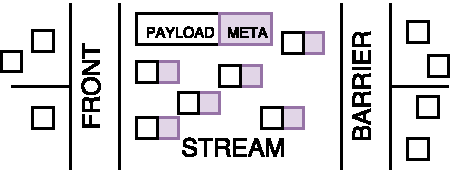
\includegraphics[width=0.48\textwidth]{pics/stream}
  \caption{Data flow}
  \label {stream}
\end{figure}

\subsection{Computaion flow}

The stream between front and barrier is handled by a directed data flow graph. Each node of the graph represents single operation, which can have multiple inputs and outputs. Edges indicate the order of these operations. Data items are processed one-by-one in a "streaming" manner. The figure~\ref{logical-graph-figure} shows the example of data flow graph.

Our model allows cycles in the graph while data flow graphs are commonly assumed to be acyclic (DAGs) 
~\cite{Zaharia:2016:ASU:3013530.2934664, Carbone:2017:SMA:3137765.3137777}. Moreover, as we show further, there are cases when cycles are required, e.g. for MapReduce-based algorithms. 

\subsection{Physical deployment and partitioning}
Data flow graph is distributed among computation unit. Each computational unit in our runtime runs process called {\it worker}, and each worker executes complete data flow graph. Every worker is assigned by an integer interval. Intervals are not intersected and cover the range of 32-bit signed integer.

Each input of a operation is assigned by user-provided hash function called {\it balancing function}. This function is applied to the payload of data items and determines partitioning. Data items are repartitioned before each operation. After that, corresponding data item is sent to the worker, which is responsible for the computed value. Therefore, load balancing explicitly depends on the balancing functions of the operations. The balancing functions are the part of business logic, because optimal balancing requires the knowledge of payload distribution. Possible partitioning of this graph on two nodes is shown on the figure~\ref{physical-graph-figure}.

\begin{figure}[htbp]
  \centering
  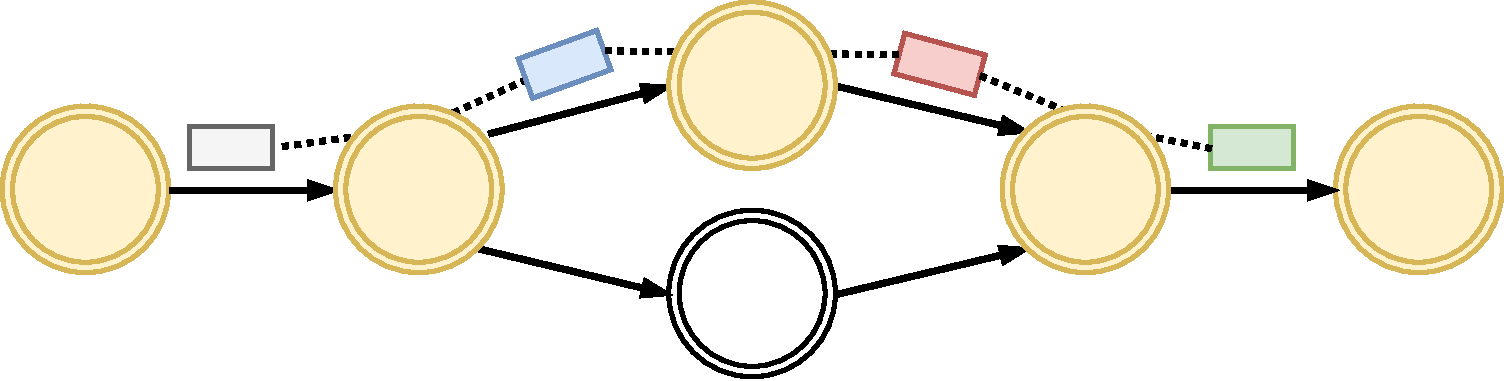
\includegraphics[width=0.48\textwidth]{pics/logical-graph}
  \caption{An example of the data flow graph}
  \label {logical-graph-figure}
\end{figure}

\begin{figure}[htbp]
  \centering
  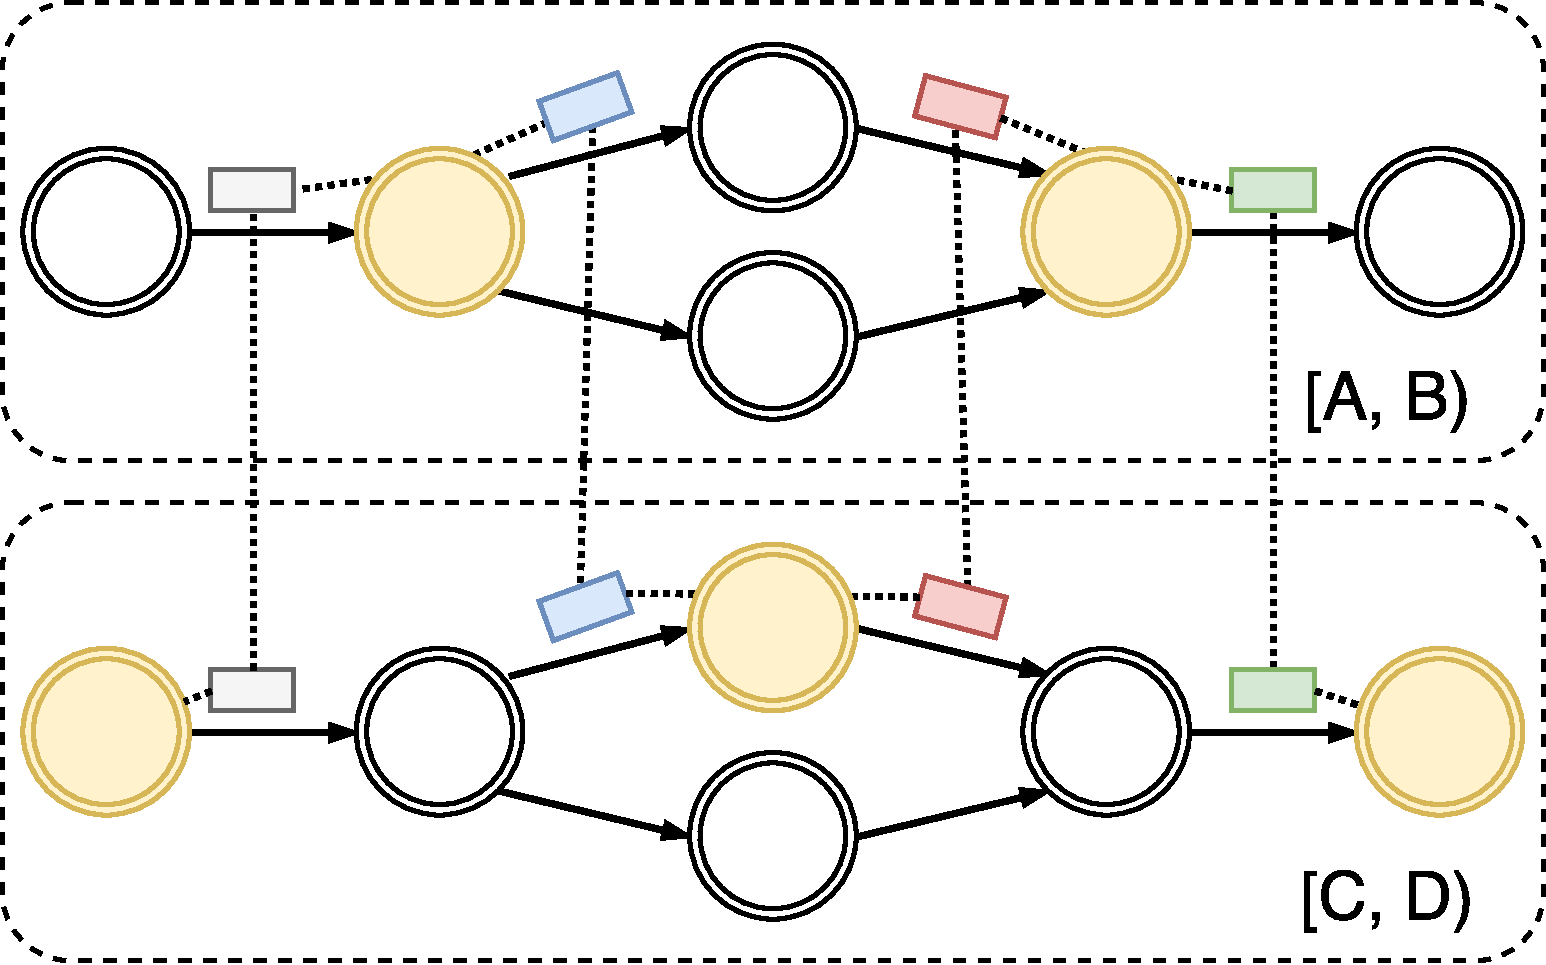
\includegraphics[width=0.48\textwidth]{pics/physical-graph}
  \caption{Possible partitioning of the data flow graph}
  \label {physical-graph-figure}
\end{figure}

\subsection{Ordering model}

As it was mentioned above, meta-information imposes an explicit total order on data items. Without diving into the details, it should be noted that the order of items is maintained across different fronts.

Let {\it image} be an output data item of an operation and {\it preimage} is a corresponding input item. In this terms, the order of images is preserved, i.e. the order of images is the same as the order of preimages. Moreover, the image of the item follows its preimage but precedes the next item. The concept of ordering is shown on the figure <>.

We assume that input items of the operations are strictly ordered. After the meta-data is assigned to data item at the front, the rest of computations become deterministic.

\subsection{Operations}

The set of available operations is limited by the following list.

{\bf Map} applies user-defined function to the payload of an input item. This function returns a sequence of data items with new payloads.

{\bf Broadcast} replicates an input item to the specified number of operations or sinks. 

{\bf Merge} operation is initialized with specified number of input nodes. Each input item from all inputs copied to the single output.

{\bf Grouping} has a {\it window size} parameter. Grouping stores input items in distinct buckets by the value of the input balancing function applied to payload. When the next item arrives to the grouping, it is appended to the corresponding bucket. Each time item grouping outputs window-sized {\it tuple item}, which consists of the last items of this bucket. The data items within tuple are ordered by the meta-information. If the size of bucket is less than window, all items of the bucket are taken. Grouping is the only operation that maintains state. To prevent collisions user can define equivalence relation to ensure that items with distinct payloads are got in the distinct buckets.

The following example illustrates the semantics of the operation. The grouping accepts items with payload represented as natural numbers: 1,2,3, etc. The hash function returns 1 if the number is even and 0 otherwise. If the window is set to 3, the output is:

\[(1), (2), (1|3), (2|4), (1|3|5), (2|4|6), (3|5|7), (4|6|8)...\]

The important property of the grouping is that the result is uniquely determined by the last element in the tuple. Therefore, grouping is the bijective mapping. Additionally, the results among items with different values of hash function are independent.

\subsection{User-defined parameters}

User is able to set up the following parameters:

\begin{enumerate}
  \item{Computation flow}
  \item{Balancing functions of the inputs}
  \item{Map functions}
  \item{Grouping windows}
\end{enumerate}

This parameters can produce more than one graph, which can yield equivalent results. Choosing among them is a performance optimization problem.    

It is important to mention, that there are no parameters for state-management. Therefore, business-logic is stateless. Nevertheless, the operations set is enough to implement any MapReduce transformation.


\section {Graph and partitioning}
%%%% fs-run-time-graph  Graph and its partitioning

\label {fs-graph}

In our model the dataflow is represented by a directed graph. This graph does not contain information about physical deployment, so further we call it {\it logical} graph. Each other node of the logical graph contains single operation, also called job or procedure. Edges show the order of these operations. The data items are processed one-by-one in a "streaming" manner.

Notably, despite the fact that commonly dataflow graphs assumed to be acyclic (DAGs) 
~\cite{Zaharia:2016:ASU:3013530.2934664, Carbone:2017:SMA:3137765.3137777},
our model does not have this restriction. Moreover, as we show further in this section, there are cases when cycles are required, e.g. for MapReduce-based algorithms. 

\subsection{Physical deployment and partitioning}

Each computational unit in our distributed runtime is assigned by integer interval. Intervals are not intersected and cover the range of 32-bit signed integer. Moreover, each unit contains complete logical graph.

Physical graph extends logical one by assigning hash function to each input of each operation. This hash function is applied to the payload of data items and determines partitioning. More precisely, the value of hash function is computed before next operation and corresponding data item is sent to the unit which is responsible for the computed value. Therefore, load balancing explicitly depends on the hash functions of the operations. Optimal balancing requires the knowledge of payload distribution. Hence, the hash functions are assigned by business logic.

Figure~\ref{logical-graph-figure} shows the example workflow of logical graph. Possible partitioning of this logical graph on two nodes is shown on the figure~\ref{physical-graph-figure}.

\begin{figure}[htbp]
  \centering
  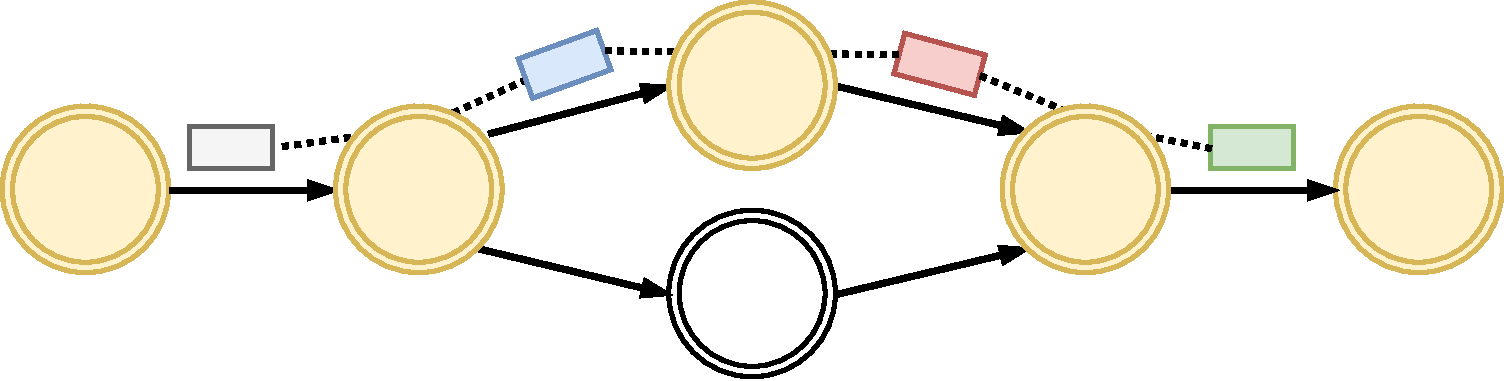
\includegraphics[width=0.48\textwidth]{pics/logical-graph}
  \caption{Logical graph workflow}
  \label {logical-graph-figure}
\end{figure}

\begin{figure}[htbp]
  \centering
  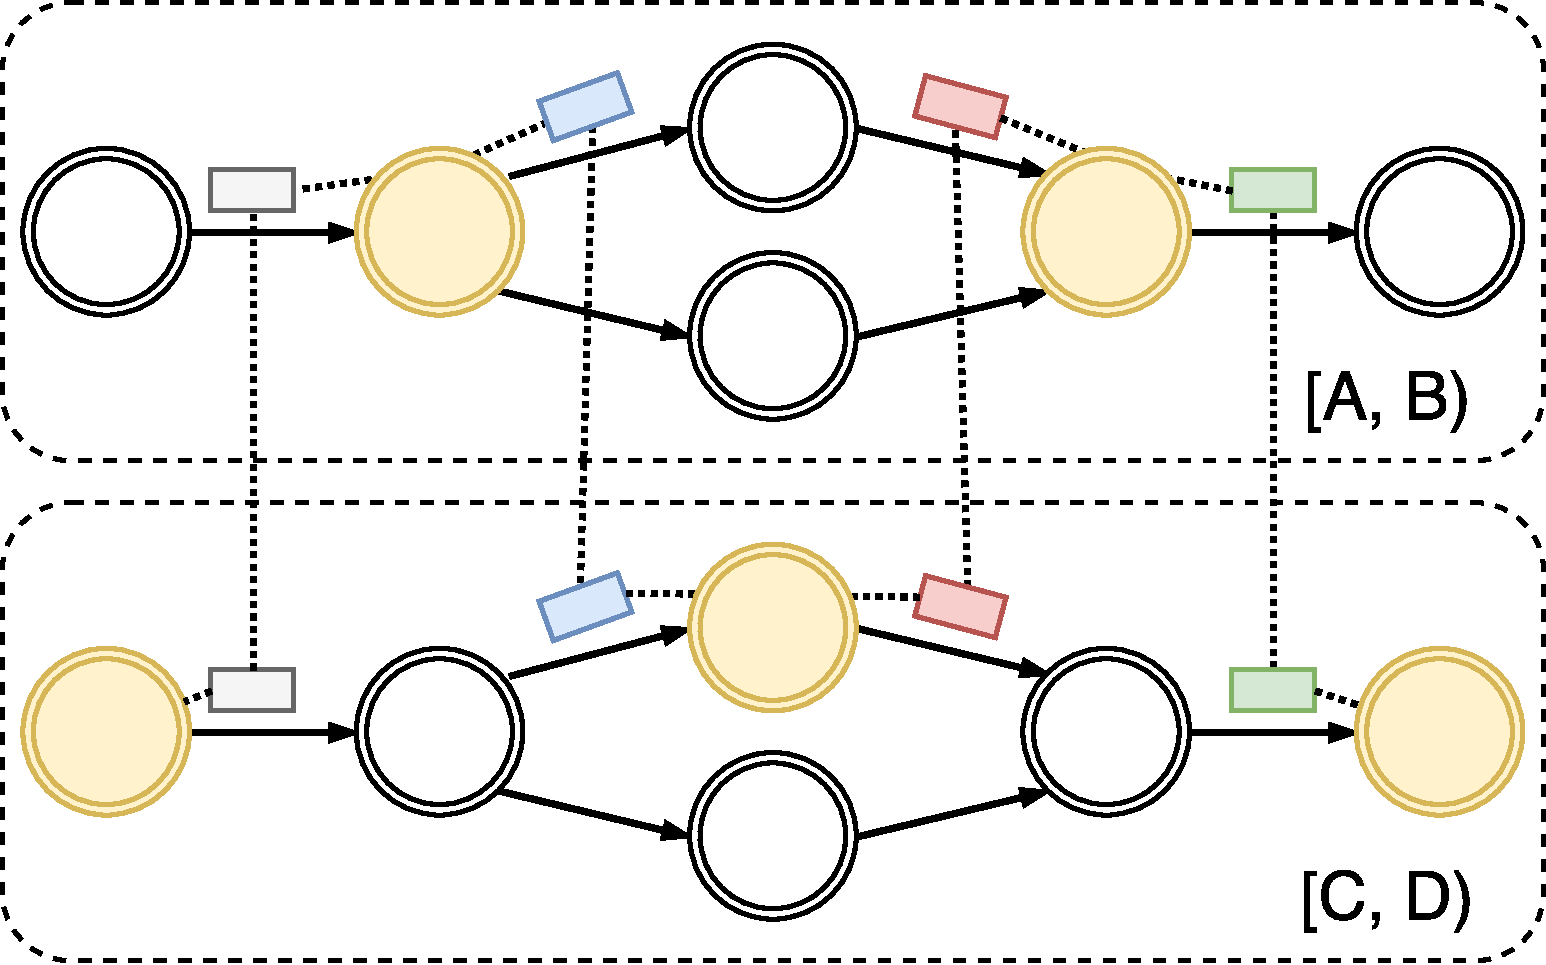
\includegraphics[width=0.48\textwidth]{pics/physical-graph}
  \caption{Possible partitioning of the logical graph}
  \label {physical-graph-figure}
\end{figure}


\section {Timing model}
%%%% fs-run-time-timing Timing model

\label {fs-timing-model}

There is an explicit total order on dataitems. Once element is produced at front it is assigned a GlobalTime, current wall-clock of the front. This allows to order items across different fronts. This ordering is preserve even after operations that is the order of images is the same as order of preimage. Moreover the image of the first element is greater than its preimage but less than the second element. It is shown on figure 7.


The semantic of operation asume that input elements are strictly ordered. The particular form of meta-information that has such ordering properties is shown in the following sections.

It is worth mentioning that after assigning the GlobalTime at the front the rest of computations is determined.


\section {Operations}
%%%% fs-run-ops Operations

\label {fs-ops}

The set of available operations is limited by the following list.

{\bf Map} applies user-defined transformation to the payload of input item. 

{\bf Flat map} applies user-defined function to the payload of input item. This function returns a sequence of new payloads. Each of these payloads is put into distinct data item. 

{\bf Filter} applies user-defined predicate to the payload of input item. If the result of predicate is positive, filter outputs initial item with updated trace of local times. Otherwise, filter outputs nothing.

{\bf Broadcast} replicates input item to the specified number of operations or sinks. 

{\bf Merge} operation is initialized with specified number of input nodes. Each input item from all input nodes is sent to the single output. It preserves ordering between input items.

{\bf Grouping} has two parameters: number called {\it window} and hash function. Grouping stores input items in distinct buckets by the value of the hash function applied to payload. When next in turn item is got in the grouping, it is put to the tail of corresponding bucket. After that, grouping outputs window-sized {\it tuple item}, which consists of the last items of this bucket. If the size of bucket is less than window, all items of bucket are taken. Notably, grouping is the only operation that maintains state.
	
Here and elsewhere, we assume that hash functions in grouping are perfect, i.e. do not have any collisions. However, practically, user can define equivalence relation to ensure that items with distinct payloads are got in the distinct buffers.
	
To completely clarify the semantics of this operation, consider the following example. The grouping accepts items with payload represented as natural numbers: 1,2,3, etc. The hash function returns 1 if the number is even and 0 otherwise. If the window is set to 3, the output is:

\[(1), (2), (1|3), (2|4), (1|3|5), (2|4|6), (3|5|7), (4|6|8)...\]

The important property of the grouping is that the result is uniquely determined by the last element in the tuple. Therefore, grouping is the bijective mapping. Additionally, the results among items with different values of hash function are independent.

\subsection{User-defined parameters}

\begin{enumerate}
  \item{Map function}
  \item{Flatmap function}
  \item{Filter predicate}
  \item{Grouping window}
  \item{Grouping hash function}
  \item{Hash-partitioning function of the inputs}
  \item{Graph itself: vertexed and edges}
\end{enumerate}

Grouping hash can be inherited from its input partitioning. Note, that non of this paramiters contains state-management. Therefore, business-logic is stateless. Despite this it is enough to implement MapReduce transformations of the stream.


\section {MapReduce transformations on stream}
%%%% fs-run-mapreduce MapReduce transformation on stream

\label {fs-mapreduce}

\begin{figure}[htb]
  \centering
  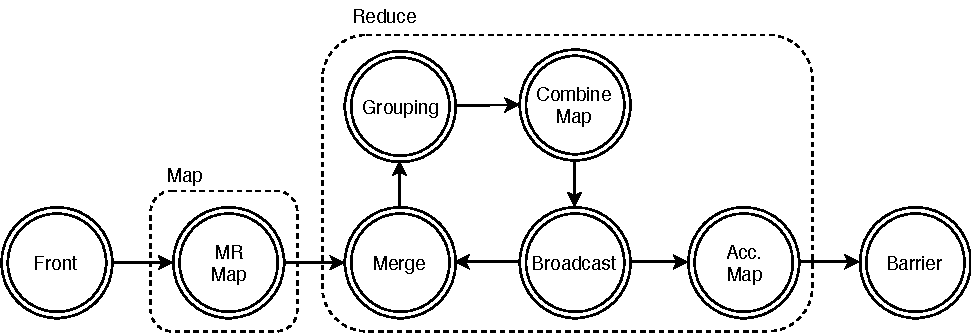
\includegraphics[scale=0.5]{pics/mapreduce}
  \caption{Logical graph for MapReduce transformations}
  \label {mapreduce-graph-figure}
\end{figure}

To show soundness of our model we demonstrate a way to implement MapReduce-like transformation of a stream. Map stage of MapReduce is directly mapped on map operation that extracts a key, but there is a complication with reduce step. Reduce step requires an explicit statate handling. The typical pseudo-code of reduce step is shown on figure 17. It need to store and update current word count.

One possibilitly to implement reduce step in out model is to make business logic state a part of a stream, and work with it as with an ordinary dataitem. Figure~\ref{mapreduce-graph-figure} shows a graph that produces reduced items. Map and reduce parts are highlited with dashed line.

Data items of this stream are: {\it input} items, {\it mapped} items, and {\it reduced} items. Each type of item and the way they were generated are detailed further in this section. However, it is worth to mention that mapped and reduced items have key-value structure of payload. The operations of the stream have the following properties:

\begin{itemize}
\item The first map operation accepts input items and outputs mapped items, according to the business logic. This operation is semantically matched with map step of MapReduce model. Additionally, it should be noted that stream onwards can contain only mapped and reduced items.
\item Merge operation is used for cycle implementation.
\item The window of grouping is set to 2. The hash function is designed to return distinct values for payloads with distinct keys.
\item Filter operation removes tuples with structure \textit{(mapped item; reduced item)}, i.e. tuples, where mapped item was generated before reduced item.
\item The all possible inputs of the second map are the following tuples: \textit{(mapped item), (mapped item; reduced item)}. Any other tuples cannot get in this map because of the filter operation and assumption about the order of items which get in grouping. The first type of input tuples is transformed into reduced item with key inherited from mapped item and some initial value.  The second type is combined into reduce item with the same key. The value of this item is the result of specified reduce function applied to the values of tuple items. Actually, this transformation is equivalent to the reduce step of MapReduce model.
\item Broadcast operation is used to return actual reduced item to grouping and, at the same time, to output it from stream. 
\end{itemize}

According to the provided logical graph, any MapReduce transformation can be implemented using the sequence of map, merge, grouping, filter, and broadcast operations. The key idea is that each reduced item always arrives at grouping right after already combined mapped item and before new one. Hence, each mapped item would be grouped with the actual reduced item. Additionally, when filter accepts tuple {\it (mapped item; reduced item)}, then it means that mapped item was generated before reduced item, and therefore, it had been already combined into the reduced item. The cycle gives ability for new reduced items to get back in grouping operation. Thereby, the stream reacts to each input item by generating new reduced item, which contains the actual value of the reduce step. 

The example of input/output items, which are generated/ transformed by the part of the logical graph, is shown on the figure~\ref {word-count-figure}. This example represents classical MapReduce-based algorithm for word counting. Map step of this algorithm transforms each input word into key-value pair where word is the key, and the value is 1. Reduce step sums all values into the final result for specific key. According to our graph for MapReduce transformations, the item {\it m[dog, 1]} represents mapped item with key "dog" and value 1. The item {\it r[dog, 1]} describes reduced item with key "dog" and value 1. The figure shows how the model reacts on two consequent input items containing word "dog". The meta-information of items is omitted for simplification. More precisely, there are shown 4 stages separated by dotted lines:

\begin{enumerate}
    \item New mapped item with key "dog" arrives at grouping with empty state. Grouping outputs tuple with this single item. Filter accepts the tuple, and Map transforms it to the first reduced item for key "dog" and value 1.
    \item The reduced item arrives at grouping after it went through the cycle. It is grouped in tuple with mapped item that has been already in the state with key "dog". However, filter drops this tuple, because of the order of items.
    \item New mapped item with key "dog" arrives at grouping. It is inserted right after the reduced item in the bucket for key "dog". Grouping outputs tuple containing the reduced item and new mapped item. Filter accepts this tuple, because it has the right order. Map operation combines reduced and mapped items into new reduced items with key "dog" and value 2.
    \item New reduced item arrives at grouping through the cycle, but new generated tuple is not accepted by filter, as well as in the step 2.
\end{enumerate}

\begin{figure}[htb]
  \centering
  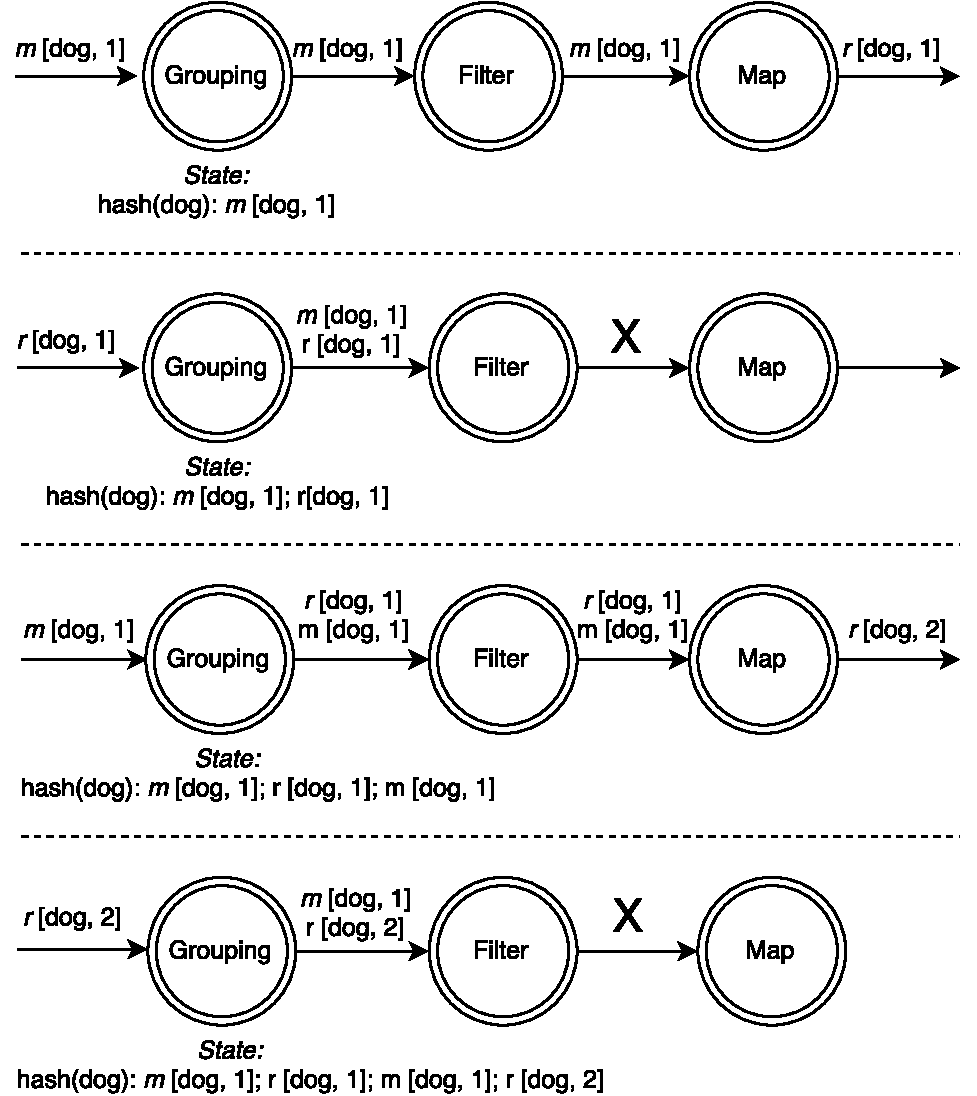
\includegraphics[scale=0.5]{pics/wordcount}
  \caption{Part of the stream evalutaion for word counting}
  \label {word-count-figure}
\end{figure}



\section {Optimistic collision management}
%%%% fs-run-mapreduce Optimistic collision management
\label {fs-collision}

As it was defined previously, only the grouping operation maintains a state and the state depends on the order of incoming items. Because of asynchrony and the possible existence of multiple paths between two nodes it is hard to deliver the right order.

In order to address this issue, we accept the fact that grouping can produce incorrect tuples. However, we guarantee that all correct tuples are eventually produced. The correctness of tuple means that this tuple would be generated if the order assumption was satisfied. 

To eventually produce all correct tuples, we use an approach called {\it replay}. If an item arrives the grouping operation, according to the meta-information order, nothing is replayed and only the most recent window is produced. However, if an item is out of order, it is inserted in the bucket at the correct location, and all tuples, which contain this element, are reproduced. Thereby, replay guarantees that eventually all correct tuples are generated. At the same time, for tuples, that has been produced but became invalid, {\it tombstones} are sent.

Tombstones are ordinal data items but with a special flag in its meta-information. This flag means that tuples with such meta-information are invalid, and they should not leave the system. Tombstones have the same payloads as invalid items in order to go through the same path in the computational pipeline.

The example of replay is shown in the figure~\ref{grouping-replaying}, The green item is out of order. The ouput consists of the new valid items, {\it (1, 2) and (2, 3)}, and the tombsone, {\it (1, 3)}.

\begin{figure}[htbp]
  \centering
  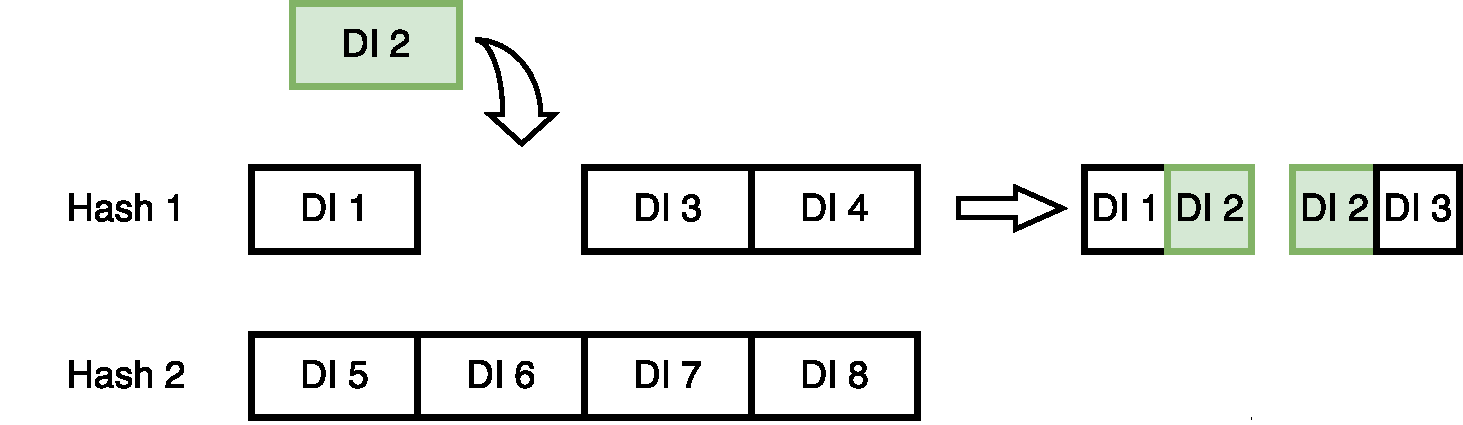
\includegraphics[width=0.48\textwidth]{pics/grouping-replaying}
  \caption{The replay in groupig with window = w. The new items are generated on insertion}
  \label {grouping-replaying}
\end{figure}

In the case of the right order of input items, there are no redundant items produced.

In order to filter out all invalid elements there is a need for {\it barrier} at the pipeline's sink, that filters invalid items when corresponding tombstones arrive. The barrier is partially flushed for some meta-information interval when there is a guarantee that there are no any out-of-order items and tombstones further up the stream for this range. The exact technique for providing such guarantee is defined further.

\subsubsection{Meta information}
The meta-information of data item is a tuple of a {\it global time}, a {\it trace}, {\it child ids} and a tombstone flag.

\[Meta := (GlobalTime, ChildIds[], Trace, IsTombstone)\]

Global time is assigned to data item once the item enters the system. It is a pair of milliseconds since the epoch start and the identifier of the front. The identifier is used to assign different global times to different items, even in case of wall-clock collisions. 

\[GlobalTime := (FrontTs, FrontId)\]

Global times are compared by front timestamp if they coincide - by front id. It is important to notice, that we are not relying on any clock synchronization between nodes, but we require a strict monotonicity within the single front. The only implication of the clock skew is the system degradation in terms of latency: 1ms of the nodes clock difference appends 1ms to minimal latency.

Each map operation can produce multiple items from one. This items are ordered between each other. To differentiate them the ordinal number, {\it child id}, is stored in the meta information. The {\it ChildIds } is an array of child ids, that corresponds to the all visited map operations.

The global time and child ids are enougth to uniquly identify data item within stream, if all processing is done without replays. If there are any replays happened during processing, multiple items with the same global time and child ids exists in the stream. There are multiple tombstones with the same global time and child ids can exist as well. They can take different paths in computational flow and travel within them with different speeds. 

Despite this fact, an invalid element and the tombstone for it are taking the same path, because they have the same payload and the balancing functions are determenistic. Moreover, the tombstome visits operations strictly after corresponding item, as links between operation are considered to be FIFO. To match tombstone with proper item there is {\it Trace} value stored in the meta-information.

Trace encodes the path item have traversed. Each phsical copy of each operation is assigned with unique random 64-bit identifier. The trace is a xor of the all operations' ids visited by item so far.

\[Trace := \bigoplus_{op \in \text{visited}} Id(op)\]

Metas are compared lexicographically. That is to say, firstly global times are compared, then child ids, then traces. Notice, this order is in line with the \FlameStream's ordering model.

The figure~\ref{logical-graph-ops-figure} shows the topology of each operation and how it affects the trace of local times.

\begin{figure}[htbp]
  \centering
  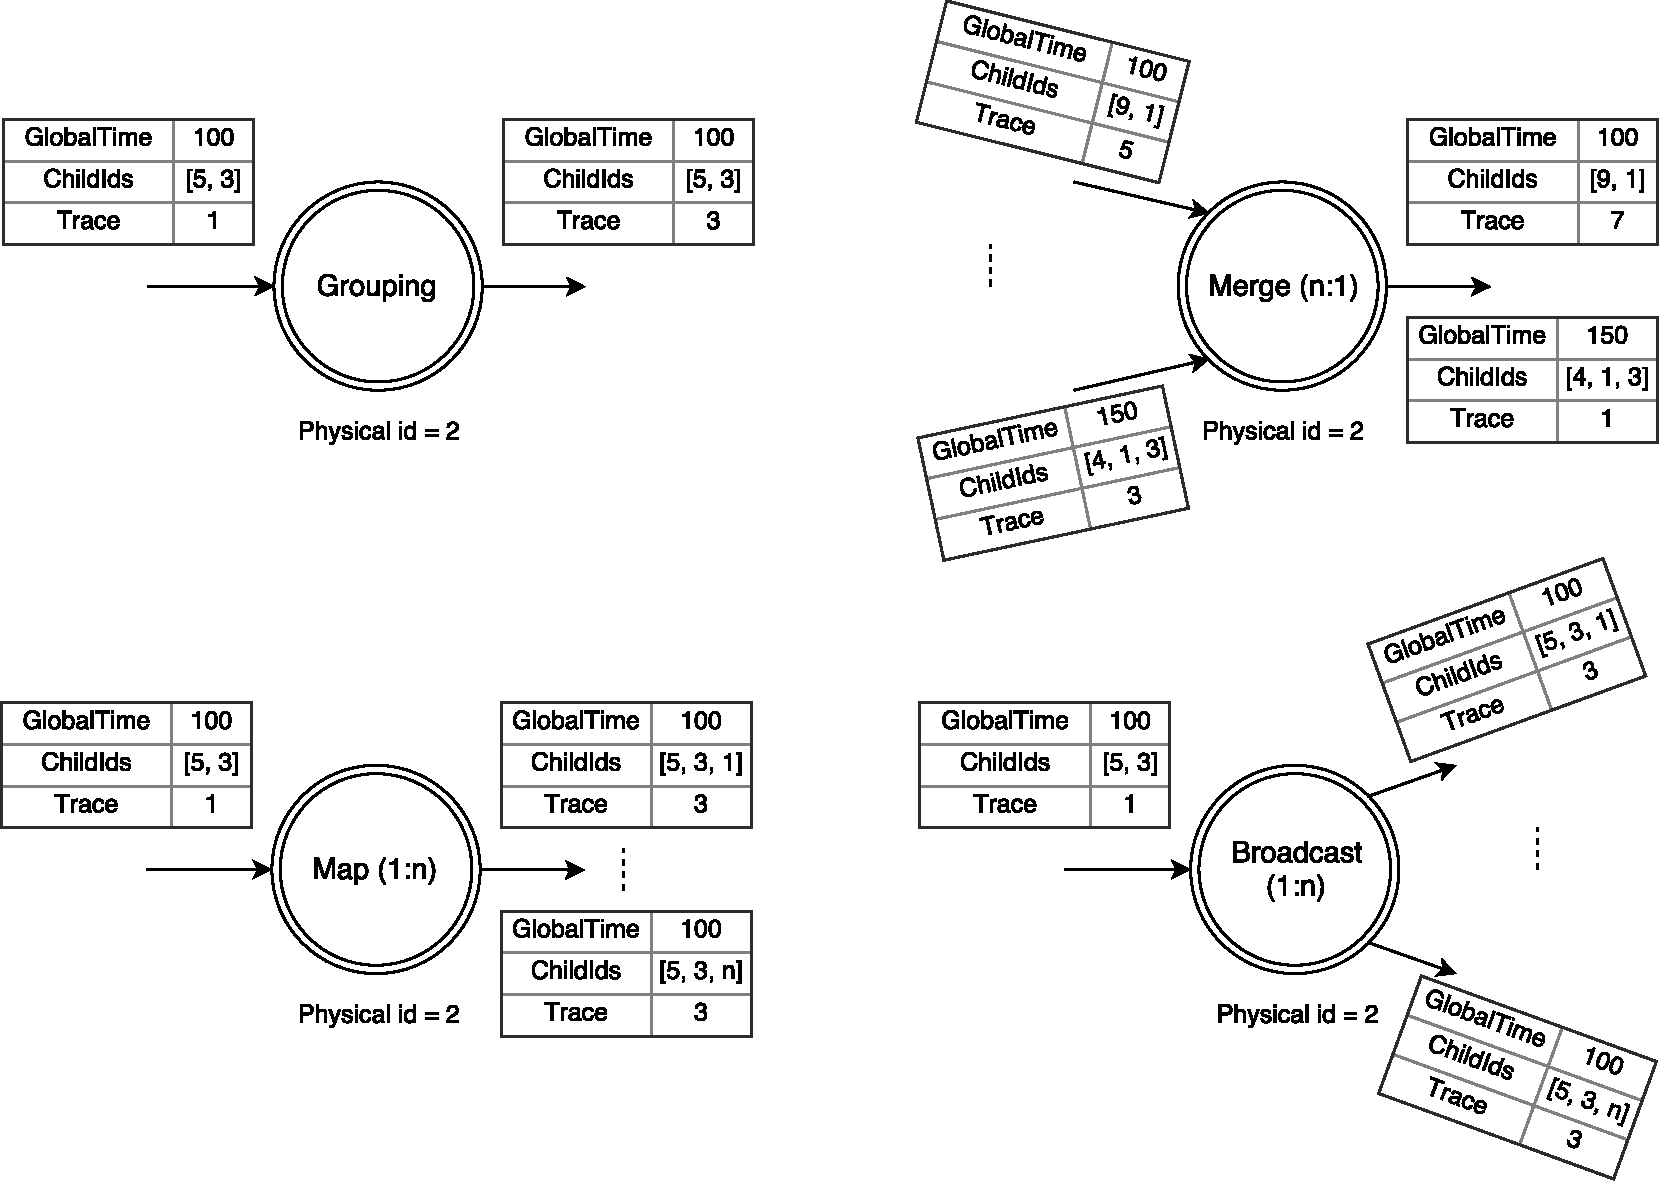
\includegraphics[scale=0.5]{pics/operations}
  \caption{Meta-information handling}
  \label {logical-graph-ops-figure}
\end{figure}

The structure of meta provides for tracking different relations between data items:

\begin{itemize}
  \item Items with same global time and common prefixes are produced from the same item
  \item Item with lower meta is generated earlier, at front or in the stream
  \item If there are two items with the same global time and child ids, only one of them is the right one
\end{itemize}

\label{mininal-time}
\subsection{Minimal time within stream}

To release the item from the barrier we need to ensure that there are no in-flight invalidators. 

\newtheorem{minimal-time-claim}{Lemma}

\begin{minimal-time-claim}
  If data item {\it D} has global time {\it GT} greater than the global time of the in-flight elements, then all tombstones for that item had already arrived at the barrier.
\end{minimal-time-claim}

\begin{proof}
  {\it RETHINK}
  Let {\it E} is in-flight element that invalidates {\it D}. According to the definition of invalidation order, {\it E} and {\it D} has the same global time {\it GT}, but the tombstone flag. We assumed that there are no in-flight element with the global time equal to {\it GT}. Contradiction.

  This implies that if the stream does not contain items with the global time less than or equal to {\it GT}, then all items which invalidate {\it D} had already arrived at the barrier. 
\end{proof}

Therefore, to output an item from the barrier, we should ensure that there are no items in the stream with the global time less than or equal to the global time of this item.

To track the global time of in-flight items we adopt an idea of {\it acker task} borrowed from Apache Storm~\cite{apache:storm}. Acker tracks data items using a checksum hash. When the item is sent or received by an operation, its global time and checksum are sent to the acker. This message is called {\it ack}. Acker groups acks by a global time into the structure called {\it ack table}. Once acker receives an ack message with global time {\it GT} and {\it XOR} it updates {\it GT} entry in the table by xoring {\it XOR} with the current value. When an item is sent and later received by the next operation, xoring corresponding {\it XOR}s would yield zero.

Acks are overlapped to nullify table's entry only when an item arrives at the barrier. That is, ack for receive is sent only after both processing and the ack sending for the transformed item, as illustrated in the figure~\ref{acker}. Different shapes of items mean different payloads. The ack for the sending of the triangular element is sent before the rectangular one. We expect the channel between the acker and each operation to be FIFO, so ack for the triangular item would be xored before the rectangular. So the two equal values are separated by distinct one. 

This technique guarantees that the {\it XOR} for some global time is equal to zero only if there are no in-flight elements with such global time.

\begin{figure}[htbp]
  \centering
  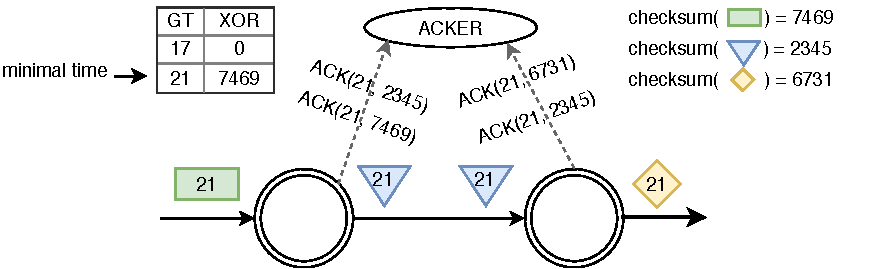
\includegraphics[scale=0.5]{pics/acker}
  \caption{Acker}
  \label {acker}
\end{figure}

The minimal time within a stream is the minimal global time with non-zero {\it XOR}. On minimal time changes, acker broadcasts new minimal time to the barrier and operations. Therefore, the barrier can release elements with global time {\it GT} once it received notification from acker that the minimal time within the stream is greater than {\it GT}.

To ensure that no fronts are able to generate item with the certain timestamp, each front periodically sends to acker special message called {\it report}, which promises that front will not generate items with a timestamp lower than the reported. The value in the ack table can become a zero only after the corresponding report arrives.

The proposed mechanism could be isolated by hash range. This change allows us making invalidation and releasing from barrier independent also known as early key availability.


\section {Barrier}
%%%% fs-run-barrier Barrier
\label {fs-barrier}

After processing, resulting items are collected in the barrier. There are valid as well as invalid ones. Its time to properly define meta-information that meets FlameStream timing model (section X) and intoduce invalidation relation that allows to distinguish valid and invalid ones.

\subsubsection{Meta information}
The meta-information of data item is represented as {\it global time} and the trace of {\it local times}.

\[Meta := (GlobalTime, Trace)\]

Global time is assigned to data item once when the item enters the system. It is represented as the concatenation of milliseconds since the epoch start and the identifier of front. Firstly, such design makes it possible to maintain global time strongly monotonic within single front. Secondly, it avoids assigning the same global time for distinct input elements. Global times can be compared lexicographically.

\[GlobalTime := (frontTs, frontId)\]

Local time is the concatenation of logical time of operation and the ordinal number of output item which we call {\it child id}. The logical time is represented as simple items counter within each operation. Therefore, child id is required, because some jobs can generate multiple items from one, e.g. flat map. The items with the same child id are called {\it brothers}. When the item leaves the operation, its trace of local times is appended by new corresponding local time. The traces of local times can be compared lexicographically.

\[Trace := [LocalTime]\]
\[LocalTime := (logicalTime, childId)\]

Notably, in spite of the fact that initially there are no items with the same global time, they can be generated by some operations. The trace of local times is used to distinguish two elements with the same global time. The main purpose of such approach is to provide information for items invalidation. The metas can be compared lexicographically: initially by global time and then by the trace of local times. 

It is important to mention that our concept of meta-information is similar to vector clocks
\cite{fidge1988timestamps, mattern88virtualtime}. However, unlike vector clocks, meta-information provides for the total order of data items due to the global time.

Figure~\ref{logical-graph-ops-figure} shows the topology of each operation and how it affects the trace of local times.

\begin{figure}[htbp]
  \centering
  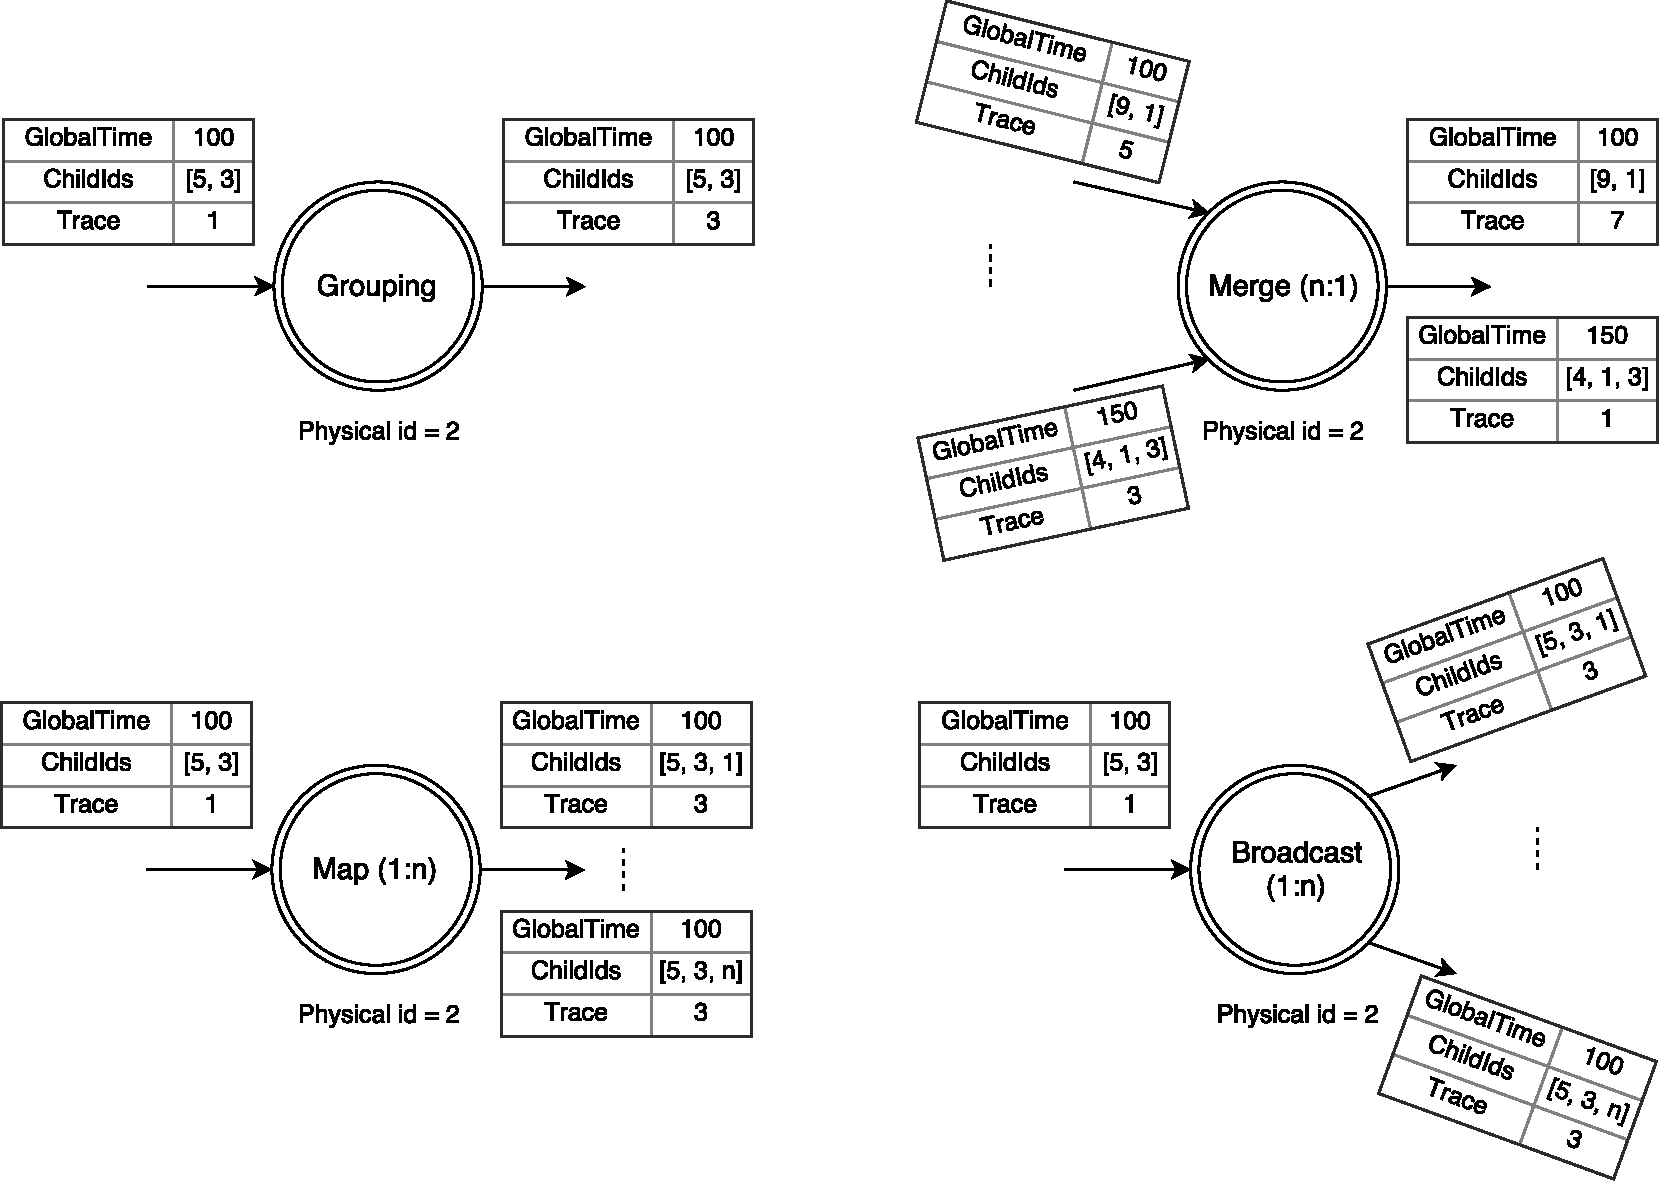
\includegraphics[scale=0.5]{pics/operations}
  \caption{Supported operations}
  \label {logical-graph-ops-figure}
\end{figure}

\subsection{Invalidation relation}

Replaying in grouping can generate incorrect tuples, multiple tuples with the same last item. Only one tuple from such set is correct. To find out which tuples are incorrect we introduce the invalidation relation between two data items. The main observation is that if there are two tuples with the same last elements, the one that the most recent on is more relevant that the previous one. 

The data item {\it A} is said to be invalidated by the data item {\it B} if:

\begin{enumerate}
\item They have the same global time
\item The trace of {\it A} is lexicographically less than the trace of {\it B}
\item The first difference is in logical time
\end{enumerate}

If the first difference is in child id, e.g. they were generated by broadcast operation, there is no invalidation relation between them. Hence, the invalidation relation is a partial order. 

Notice that the invalidation relation is defined not only on the grouping output, but on the all items. Stateless operation can not distinguish valid and invalid items and thy act on them as on the regular item. The invalidation relation cannot be lost, when item is go through other operations, because the trace of local times is append-only.

Barrier maintains a buffer for items. Once a new item arrives it inserts it in buffer and removes items that are invalidated by it.

However, there are two difficulties. Firstly, barriers are deployed on multiple workers and are partitioned by the business-logic hash function. Hence, item and corresponding invalidation item can arrive to distinct barriers. Invalidating element has the same global time as the invalidee, so the partitioning of barriers by global time solves this problem. Secondly, it is unclear when the items should be released from the barrier. To do it the system should ensure that there are no in-flight items which can invalidate items in buffer. The solution of this problem is detailed in the next section. 

Figure~\ref{invalidation-problems-figure} illustrates possible barrier issues. Red items with labels 4 and 7 got out from the system, despite the fact that they should be invalidated by corresponding green items. 

\begin{figure}[htbp]
  \centering
  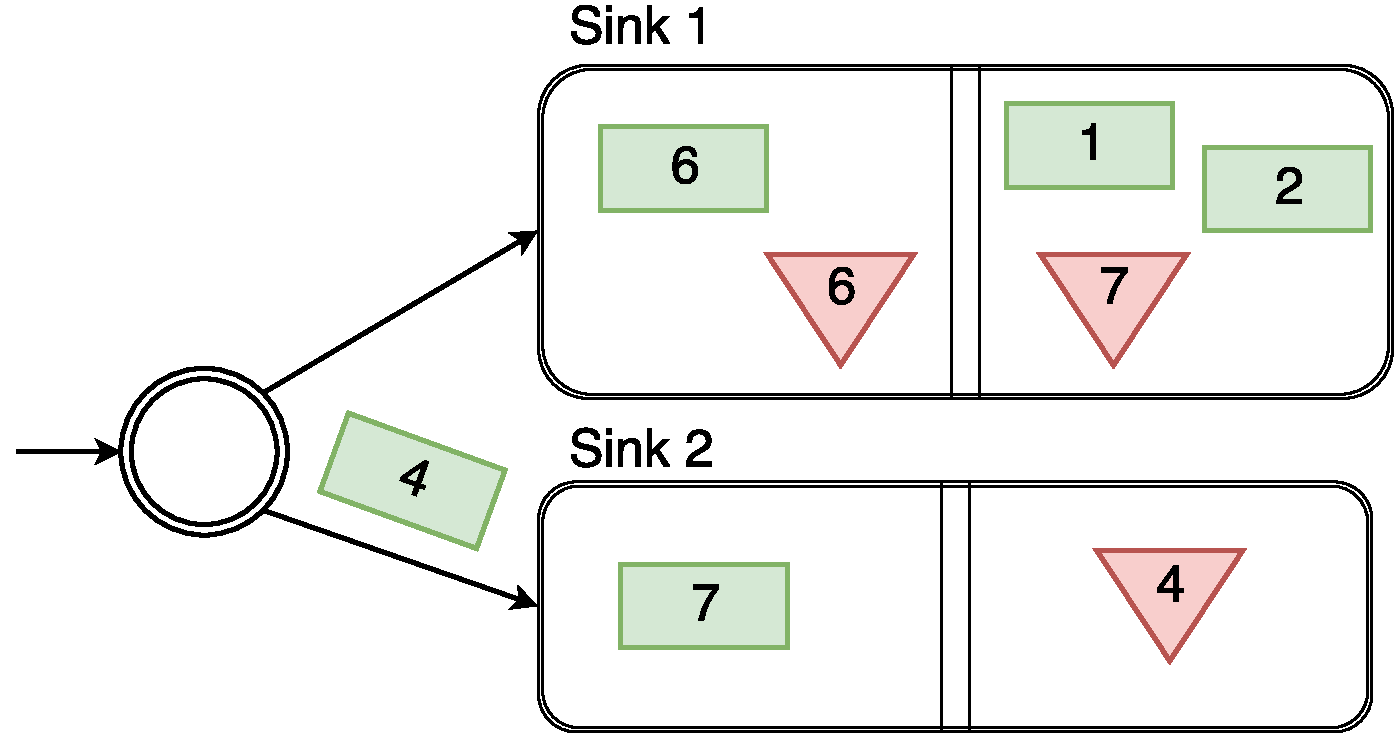
\includegraphics[width=0.48\textwidth]{pics/invalidation_problems}
  \caption{Possible barrier issues}
  \label {invalidation-problems-figure}
\end{figure}

\subsection{Minimal time within stream}
To output only correct items we need to ensure that there are no in-flight data items which can invalidate items in the barrier's buffer. In this subsection we offer sufficient condition that stream does not contain such items. Additionally, we describe how this condition is used in implementation.

\newtheorem{minimal-time-claim}{Claim}

\begin{minimal-time-claim}
Let {\it D} represent data item in barrier buffer and let {\it GT} represent its global time. If the items with global time less than or equal to {\it GT} do not exist and cannot appear in the stream, then all items that invalidate {\it D} had already arrived at the barrier buffer.
\end{minimal-time-claim}

\begin{proof}
Let {\it $D\prime$} invalidate {\it D}. According to the definition of invalidation relation, {\it $D\prime$} and {\it D} have the same global time {\it GT}, but different traces of local times. Let {\it LT} and {\it $LT\prime$} be the first distinct local times of {\it D} and {\it $D\prime$} respectively. Such difference could appear only as a result of grouping replay. Hence, {\it D} and {\it $D\prime$} are tuple items.

The global time of tuple item is inherited from the last item in the tuple, i.e. the last item in tuple {\it $D\prime$} has global time {\it GT}. Therefore, considering the properties of grouping operation, {\it $D\prime$} could be generated only if item with global time less than or equal to {\it GT} arrived at grouping. 

This implies that if stream does not contain items with global time less than or equal to {\it GT} and such items cannot appear, then all items which invalidate {\it D} had already arrived at barrier buffer. 
\end{proof}

Regarding this claim, to output item from barrier buffer we should ensure that:
\begin{enumerate}
    \item There are no items in stream with global time less than or equal to the global time of this item;
    \item Such items cannot be generated.
\end{enumerate}

To ensure that stream does not contain these items, we use module called {\it acker}. Its idea was proposed by Apache Storm \cite{apache:storm}. Acker tracks data item within the stream using a checksum hash. When item is sent or received by operation, its hash is XORed into the checksum. Therefore, if all items arrive at sink successfully, the checksum is zero. 

To find out the least global time of the items in stream, checksums are grouped by timestamps of global time into the structure called {\it ack table}. Hence, if the value of the specific timestamp in the ack table is zero, there are no items with corresponding global time into the stream. 

Notably, to ensure that no fronts would generate item with this timestamp, each front periodically sends to acker special message called {\it report}, which contains the least timestamp that can be assigned to data item by the front. The value in the ack table can become a zero only after corresponding report is arrived.  


\section {Implementation}
%%% fs-run-time-impl Implementation
\label{fs-impl}

\FlameStream\ is implemented in Java, using Akka framework for messaging. There are several main components within the implementation:
\begin{description}
  \item[Data producers and data consumers] are deployed separately and play the role of data source and data sink correspondingly.

  \item[Graph] is a component that is deployed on each node and executes a computational pipeline defined by a logical graph. Operations within the same node communicate with each other via direct function calls for performance optimization.

  \item[Barrier] filters out invalid data items. Besides, it delivers output items to data consumers.

  \item[Acker] tracks data items within the stream. Its functionality is detailed further.

  \item[Apache ZooKeeper] is used for cluster management. The usage of ZooKeeper mitigates the need for the dedicated master node.

  \item[Persistent storage] is needed for recovery in case of failures
\end{description}

The overall scheme of the system components is shown in Figure~\ref{system-architecture}.

\begin{figure}[ht]
  \centering
  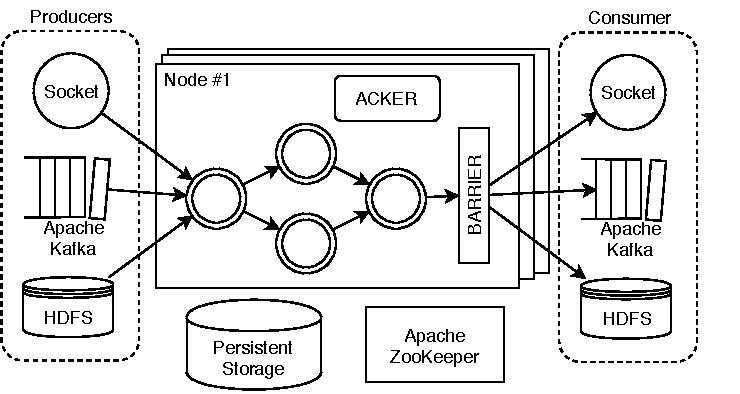
\includegraphics[width=0.70\textwidth]{pics/arch}
  \caption{The overall scheme of the system components}
  \label {system-architecture}
\end{figure}

\subsection{Ordering model}
The meta-information of data item is implemented as a tuple of a {\it global time}, a {\it trace}, {\it child ids} and a {\it tombstone flag}.

\[Meta := (GlobalTime, ChildIds[\:], Trace, IsTombstone)\]

Global time is assigned to data item once the item enters the system. It is a pair of logical time and the identifier of the front. The identifier is used to resolve time collisions within different fronts. It is important to notice that we do not rely on any clock synchronization between nodes. The only implication of the clock skew is the system degradation regarding latency: 1 ms of the fronts clock difference appends 1 ms to minimal latency.

Each map operation can produce multiple items from one.  An ordinal number, child id, is stored in the meta information to differentiate them. {\it ChildIds} is an array of child ids, that corresponds to all visited map operations.

The global time and child ids are enough to identify data item within a stream if all processing is done in-order. In this case, if we compare global time and child ids lexicographicaly the meta has the desired properties that were defined in section~\ref{model-section}. 

In order to filter out all invalid data at the barrier, there is a need to match tombstones with corresponding invalid items. However, if any grouping repairs happened during processing, multiple items with the same global time and child ids exist in the stream. To differentiate them without direct payload comparison, there is a {\it Trace} value stored in the meta-information. The trace is a xor of all physical operations' ids (random 64-bit identifier) visited by item so far. Invalid item and the corresponding tombstone go along the same path, because they have the same payload and the balancing functions are deterministic. Therefore, item and the corresponding tombstone can be revealed via trace matching. 

\label{mininal-time}

\subsection{Minimal time within stream}

To release an item from the barrier we need to ensure that there are no in-flight tombstones for that item, i.e., tombstones which have been already generated, but have not arrived at the barrier yet.

\newtheorem{minimal-time-claim}{Lemma}

\begin{minimal-time-claim}
For any data item $D$ let $\mathcal{G} (D)$ be its global time. 
  If data item $D$ has global time $\mathcal{G} (D) < \mathcal{G} (F)$ for each in-flight element $F$, 
  then all tombstones for that item had already arrived at the barrier.
\end{minimal-time-claim}

\begin{proof}
  Let $D_{tomb}$ be a tombstone for {\it D}. 
  According to the definition of the tombstone item, $\mathcal{G} (D_{tomb}) = \mathcal{G} (D)$, hence $D_{tomb}$ is not in-flight.
  
  New tombstones for $D$ cannot be generated because items with global time greater than $\mathcal{G} (D)$ cannot trigger repair that affects $D$,
  This implies that if the stream does not contain items $D\prime$ such that $\mathcal{G} (D\prime) \le \mathcal{G} (D)$, then all tombstones for $D$ had already arrived at the barrier. $\square$
\end{proof}

Therefore, to output an item from the barrier, we should ensure that there are no items in the stream with the global time less than or equal to the global time of this item.

To track the global time of in-flight items we adopt an idea of {\it acker task} inspired by Apache Storm~\cite{apache:storm}. Acker tracks data items using a checksum hash, called {\it XOR}. When the item is sent or received by an operation, its global time and checksum are sent to the acker. This message is called {\it ack}.
 Acker groups acks by a global time and xors received checksum hashes. 
When an item is sent and later received by the next operation, xoring corresponding {\it XOR}s would yield 0.

Acks are overlapped to nullify {\it XOR} only when an item arrives at the barrier. That is, ack for receive is sent only after both processing and the ack sending for the transformed item are done, as illustrated in Figure~\ref{acker}. This technique guarantees that the {\it XOR} for some global time is equal to zero only if there are no in-flight elements with such global time.

\begin{figure}[ht]
  \centering
  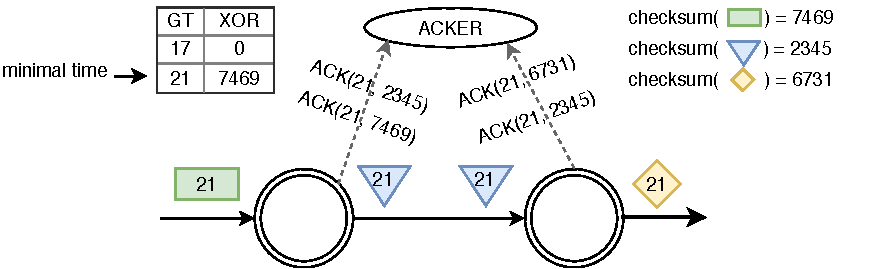
\includegraphics[width=0.8\textwidth]{pics/acker}
  \caption{The example of tracking minimal time using acker}
  \label {acker}
\end{figure}

The minimal time within a stream is the minimal global time with non-zero {\it XOR}. On minimal time changes, acker broadcasts the {\it new minimal time notification}. 
Therefore, the barrier can release elements with global time $\mathcal{G} (D)$ 
once it received notification with time greater than $\mathcal{G} (D)$.

To ensure that no fronts can generate item with the specific timestamp, each front periodically sends to acker a special message called {\it heartbeat} indicating that front will not issue items with a timestamp lower than the reported. The value in the ack table can become zero only after the corresponding heartbeat arrives.


\section {Experiments}
%%%% fs-run-time-experiments   Experiments

\label{fs-experiments-section}

\subsection{Setup}
We evaluated the series of experiments in order to estimate the performance of our system's prototype. As a stream processing task, we apply the computation of inverted index for Wikipedia documents. The computation of inverted index is implemented in terms of MapReduce transformations. We start with page mapping into the pairs {\it (word; word positions within the page)}. After that, word positions are reduced by word into the single structure. We assume the output of the stream to be change records of the inverted index structure, i.e. each input page triggers the output of the corresponding updates. 

Pairs {\it (word; word positions within the page)} must be ordered by page id and version before the update of inverted index state. Otherwise, it is possible to obtain the inconsistent index, if there are multiple versions of the same document.  
In the real-world, such scenario can be found in freshness-aware systems e.g. news processing engines. By the notion of {\it latency} we assume the time between two events: 
\begin{enumerate}
    \item Input page is taken into the stream
    \item All the change records for the page leave the stream
\end{enumerate}

In \FlameStream\ this algorithm is implemented as the typical conversion of MapReduce transformation, which is shown in section~\ref{fs-drifting}. Inverted index structure plays the role of an accumulator, and the accumulator map produces the most recent changes of this structure if any.

Our experiments were performed on the cluster of Amazon EC2 micro instances with 1GB RAM and 1 core CPU. We used 10000 Wikipedia articles as a dataset. 

\subsection{Overhead and scalability}

We take the ratio of arrived at the barrier items count to the number of the valid items among them as a key metric for the estimation of the overhead of our prototype. This value clearly represents the extra cost of our approach.

The relation between the number of workers, the delay between input documents and the proposed ratio is shown in Figure~\ref{overhead}. As expected, the peak of the ratio is achieved when the document per second rate is high, and the number of the nodes is low. This behavior can be explained by the fact that a few workers cannot effectively deal with such intensive load. Nevertheless, the proportion of invalid items reduces with the increase of workers number. Under non-extreme load, the total overhead of the optimistic approach is under 10\% for all considered number of workers. These results confirm that the ratio does not increase with the growth of the number of nodes.

\begin{figure}[htbp]
  \centering
  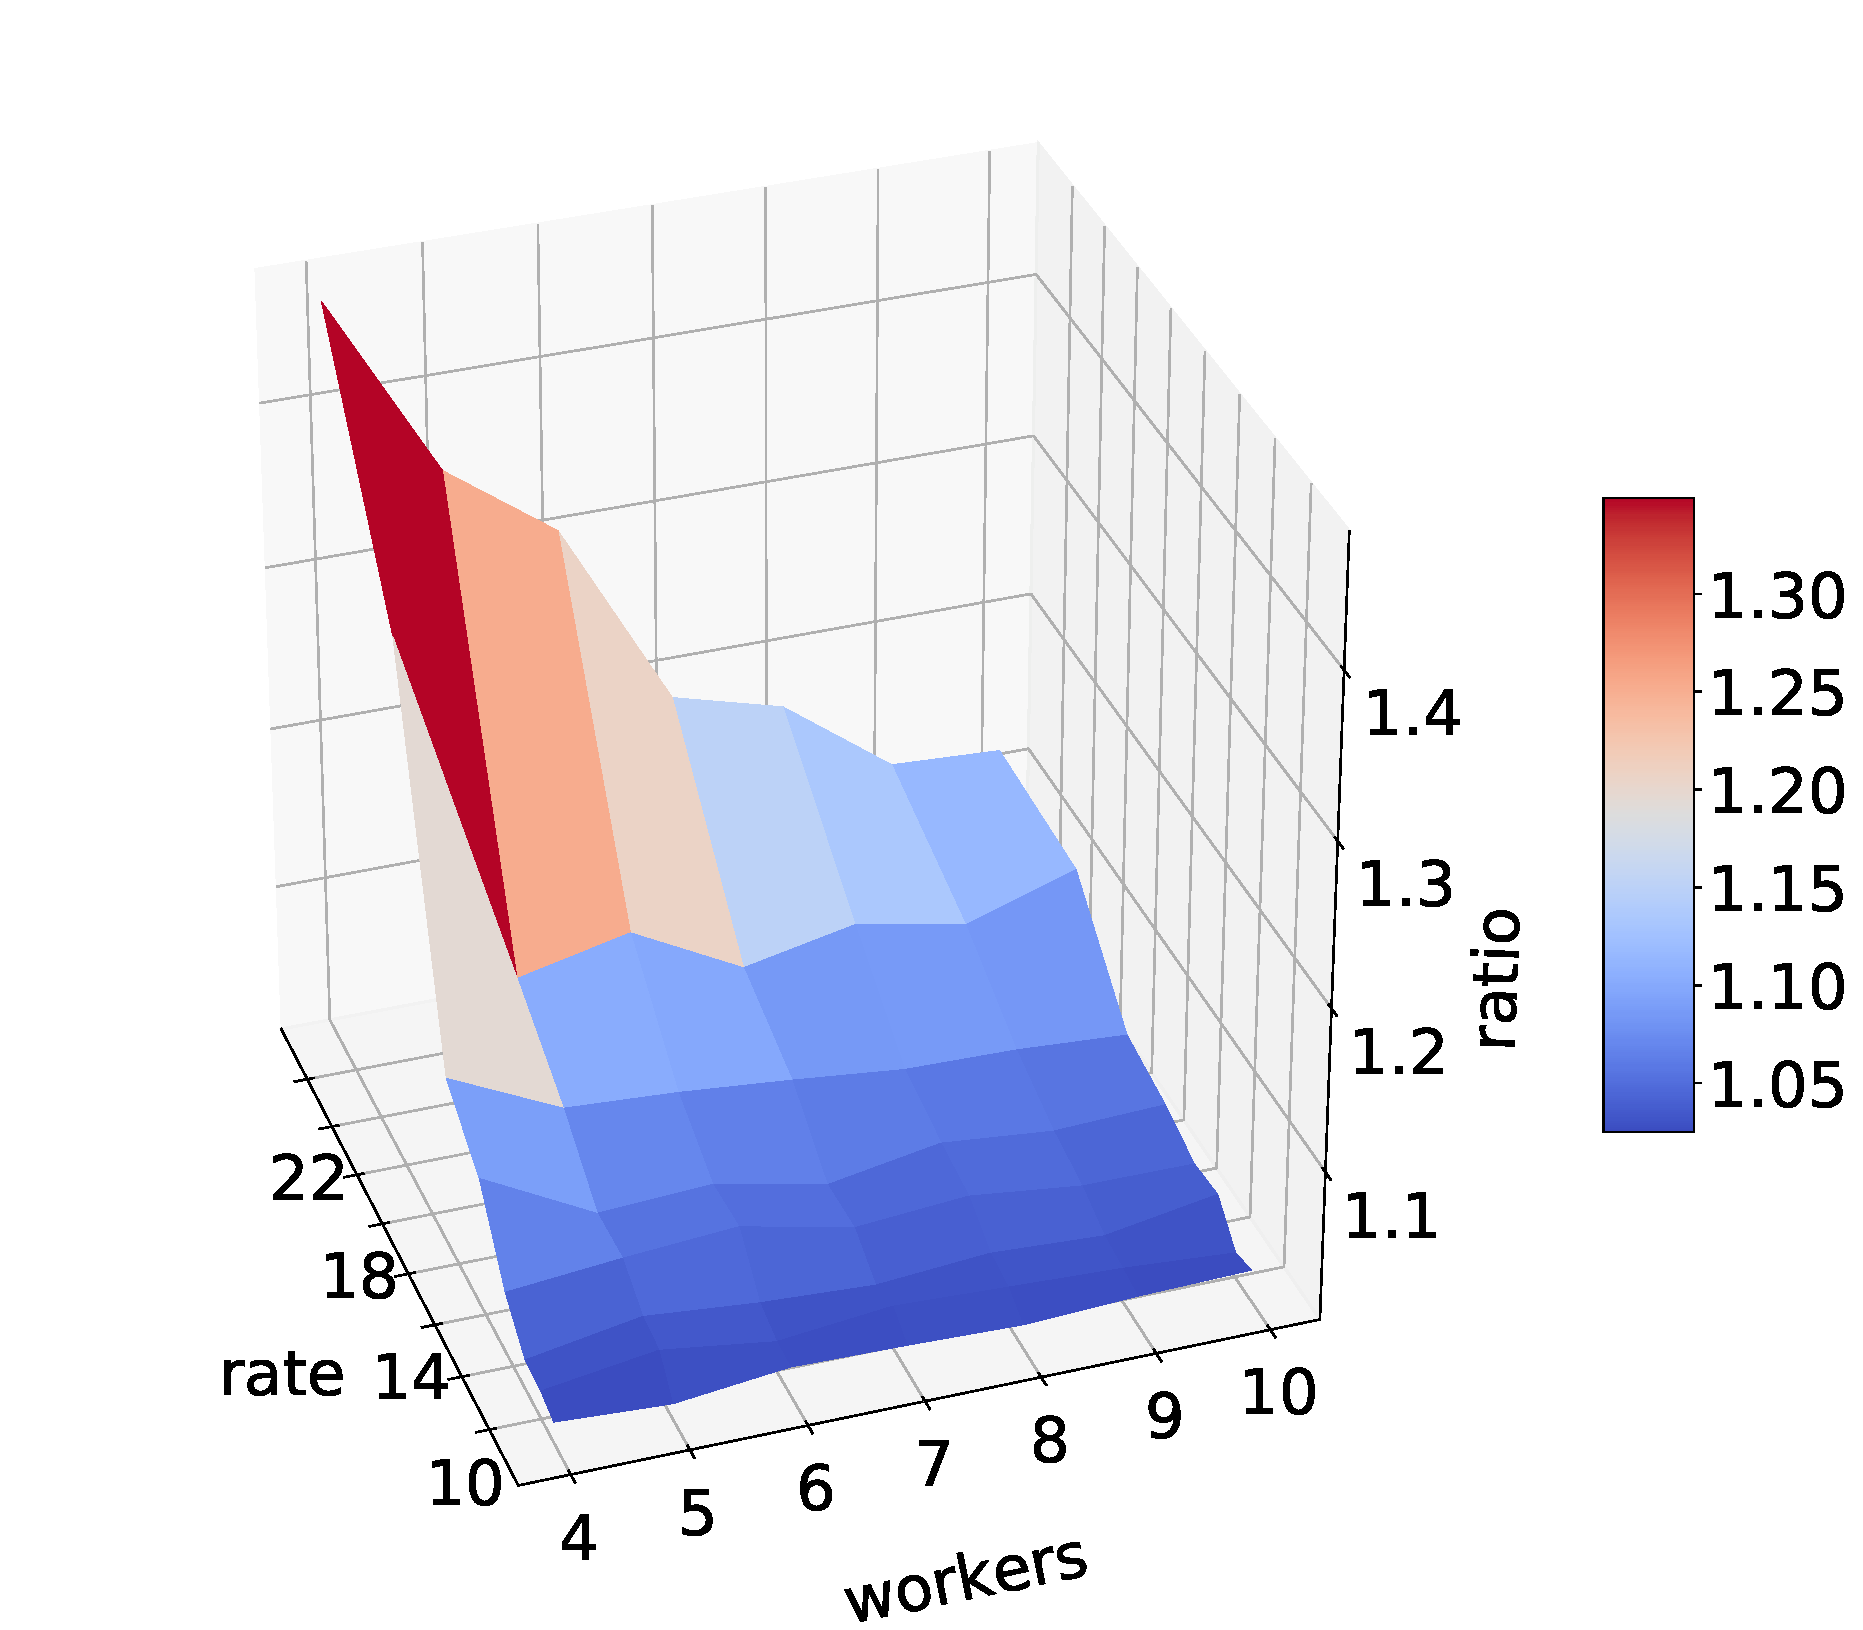
\includegraphics[width=0.5\textwidth]{pics/overhead}
  \caption{The relation between the number of workers, the delay between input documents and the replay ratio}
  \label {overhead}
\end{figure}

The latencies of \FlameStream\ across multiple workers for the fixed document rate of 70 ms are shown in Figure~\ref{fs-index-quantiles}. These figure demonstrate that latency is not significantly increased with the growth of the number of workers. 

Therefore, the most important conclusions of these experiments are: the proposed method is scalable, the overhead could be optimized by system setup.

\begin{figure}[htbp]
  \centering
  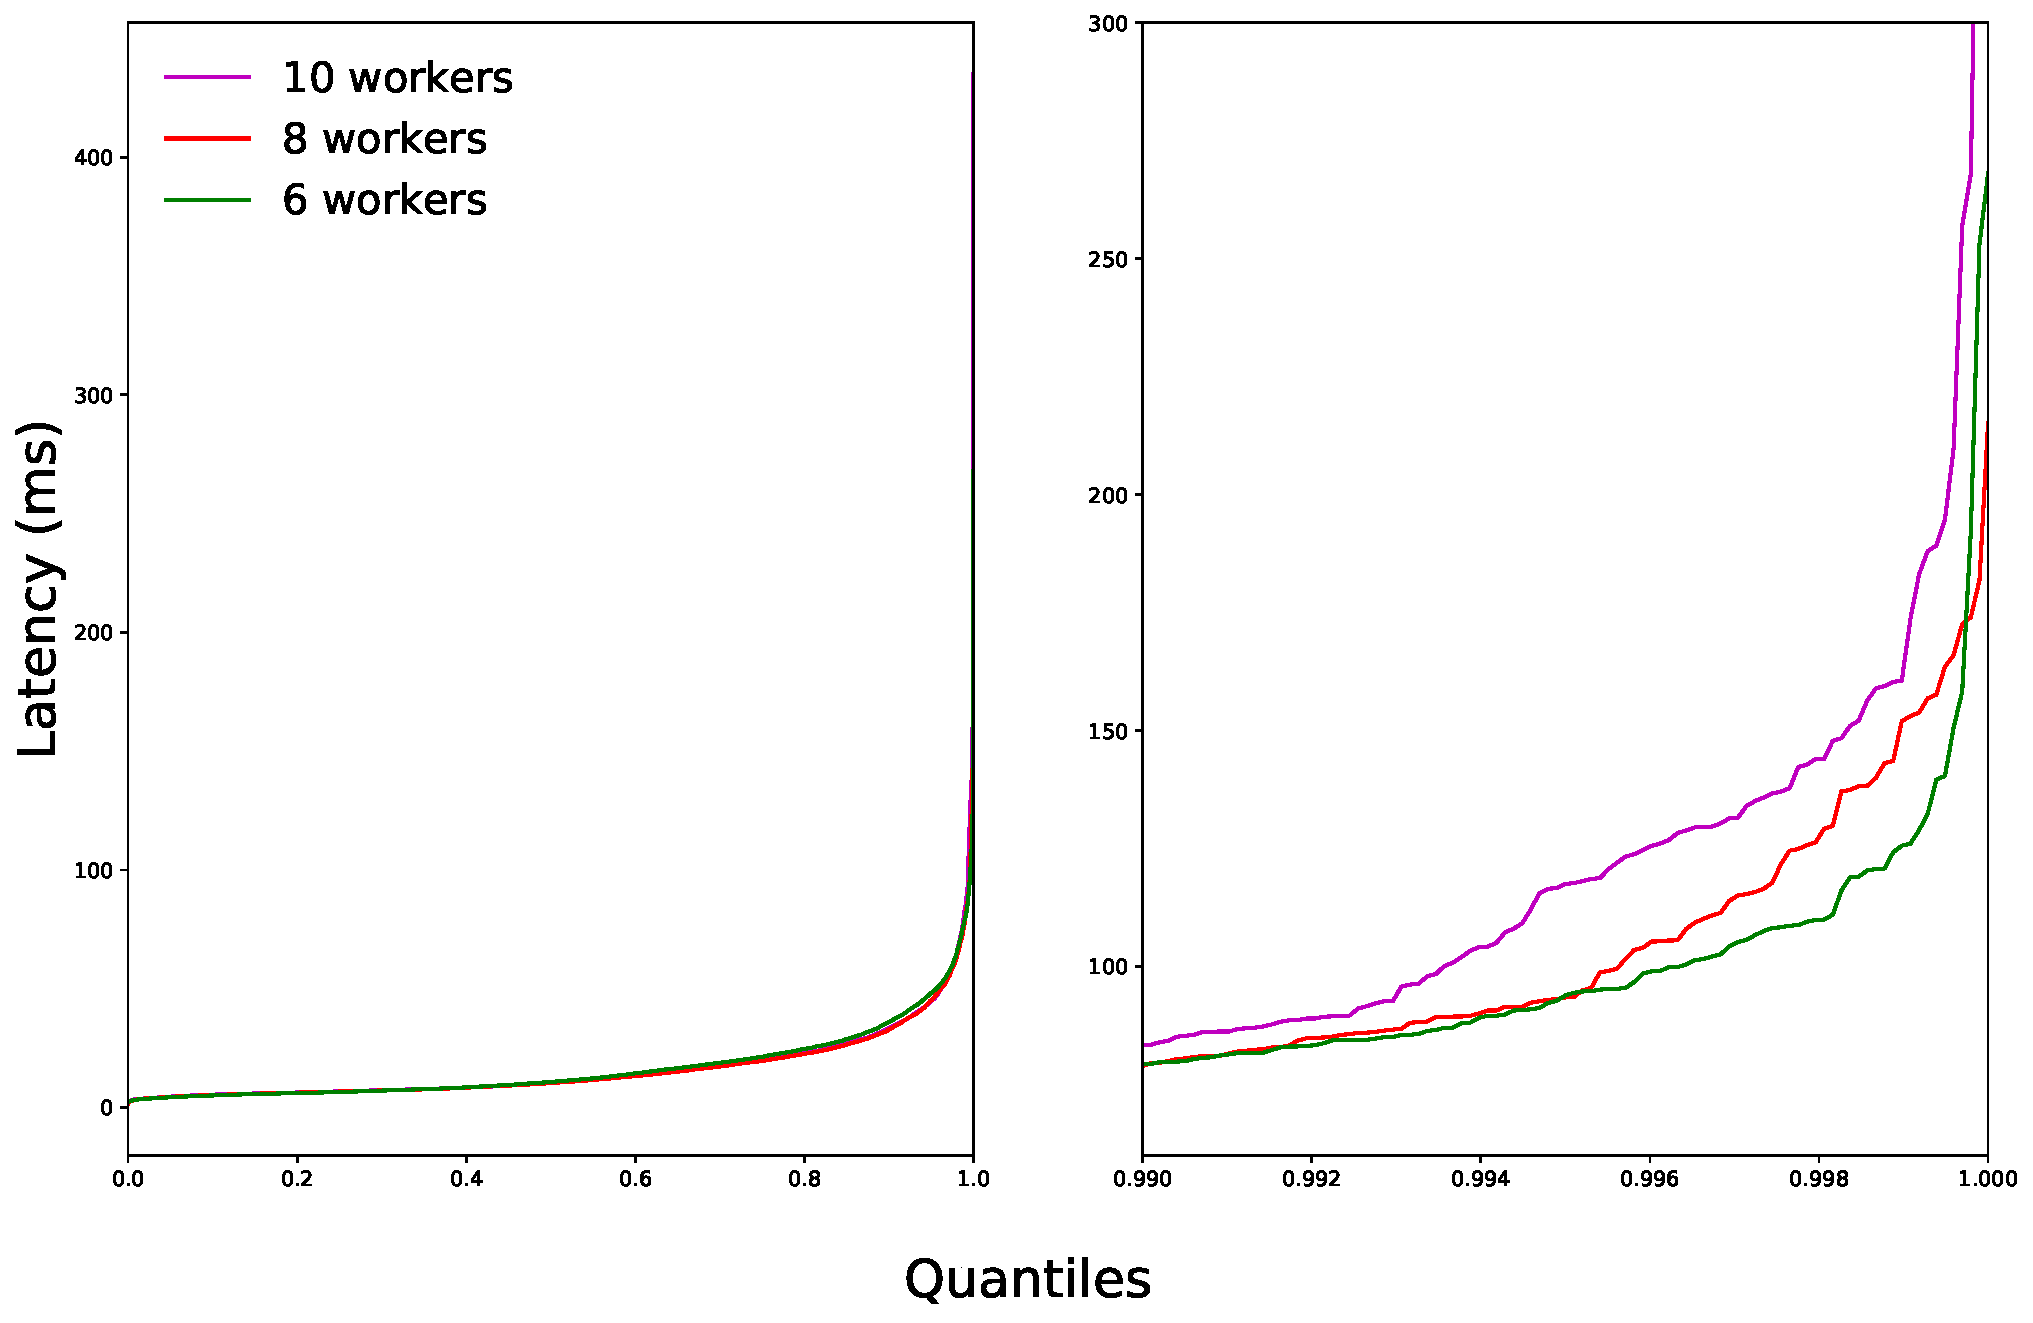
\includegraphics[width=0.48\textwidth]{pics/fs-index-quantiles}
  \caption{FlameStream latency distribution. Left - the whole distribution, right - tail latencies}
  \label {fs-index-quantiles}
\end{figure}

\subsection{Comparison against Apache Flink}

One of the most important goals of the experiments is the performance comparison with an industrial solution in terms of latency. Apache Flink is chosen for evaluation because it is state-of-the-art stream processing system that provides similar functionality and achieves low latency in the real-world scenarios~\cite{S7530084}. 

For Apache Flink, the algorithm for inverted index computation is adopted by the usage of {\it FlatMapFunction} for map step and stateful {\it RichMapFunction} for reduce step and for producing the change records. Order enforcing before reduce is implemented using custom {\it ProcessFunction} that buffers all input until corresponding low watermark is received. Watermarks are sent after each document. The network buffer timeout is set to 0 to minimize latency.

In this paper we compare $50^{th}$, $75^{th}$, $95^{th}$, and $99^{th}$ percentile of distributions, which clearly represent the performance from the perspective of the users' experience. Many papers report on averages, so these are included where it makes sense for comparison purposes. 

The comparison in latencies between \FlameStream\ and Flink within 10 nodes and distinct document rates is shown in Figure~\ref{fs-index-quantiles}. These results indicate that \FlameStream\ provides greater latency in the case of high load (25 rps). This fact corresponds with Figure~\ref{overhead}, which demonstrates that the overhead under such load is quite high. However, \FlameStream\ delivers better latency under less extreme loads. Firstly, the reason for such behavior can be the fact that Flink starts to update index only after the buffer before reduce stage is flushed. In contrast, \FlameStream\ flushes its barrier right before data is sent to a user, according to its optimistic nature. Secondly, low watermarks go along the stream and can be delayed by long-running operations, while acker processes ack messages independently. It is confirmed by Figure~\ref{buffer-vs-barrier}, which shows the comparison between waiting time in Flink's buffer and \FlameStream's barrier. 

\begin{figure}[htbp]
  \centering
  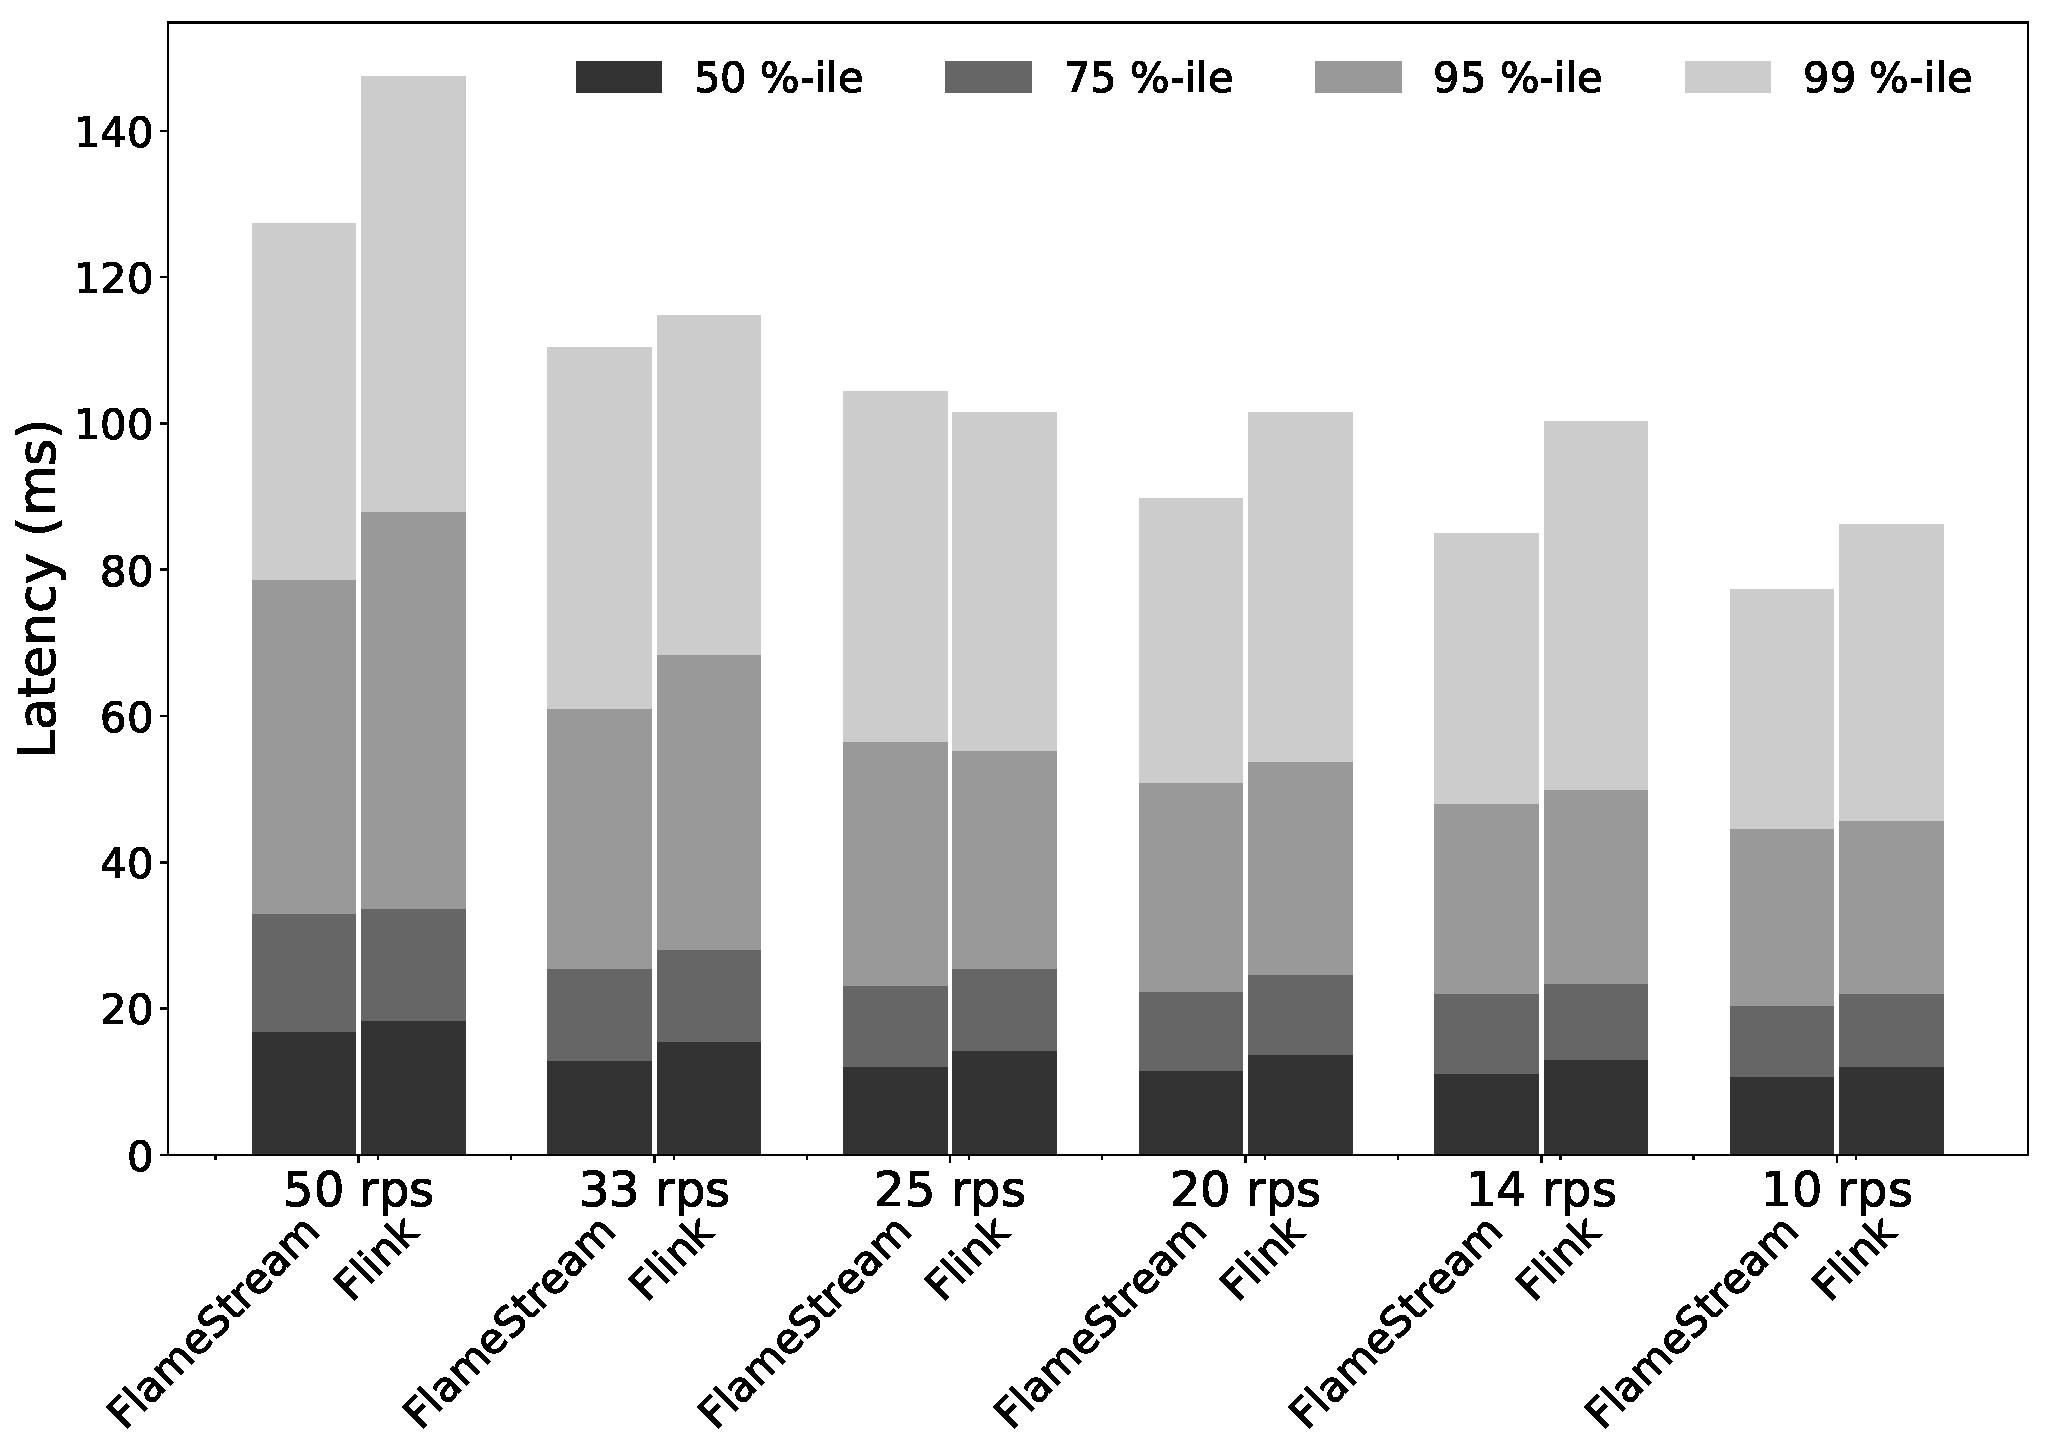
\includegraphics[width=0.5\textwidth]{pics/comp-index-quantiles}
  \caption{Latency comparison}
  \label {fs-index-quantiles}
\end{figure}

\begin{figure}[htbp]
  \centering
  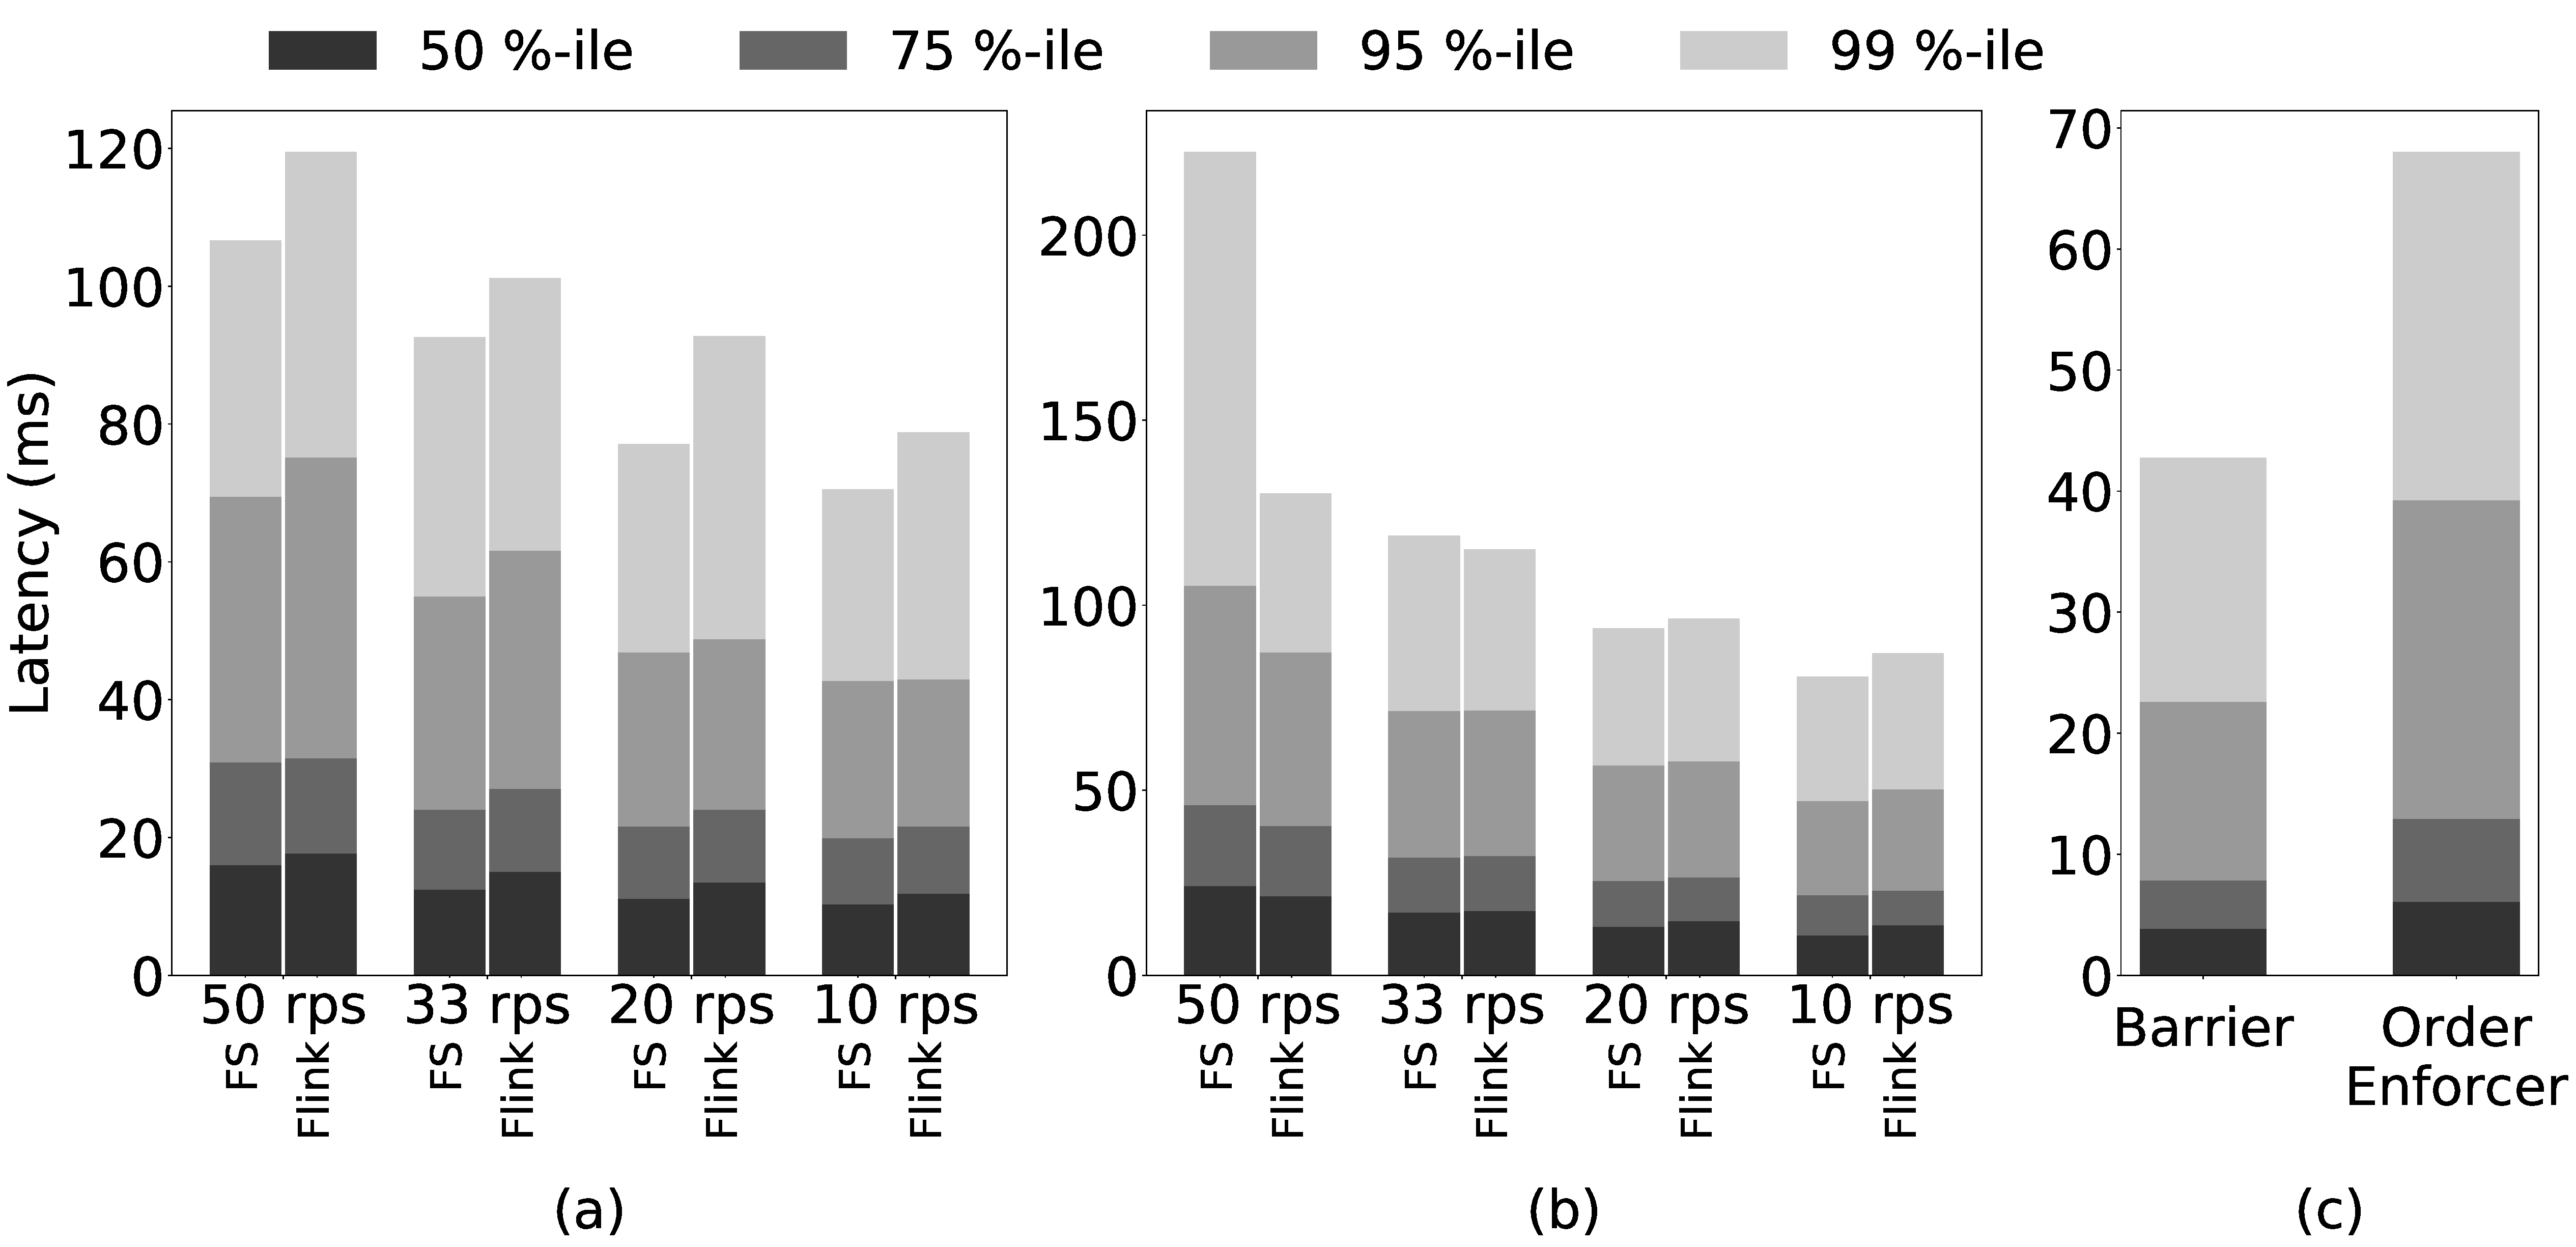
\includegraphics[width=0.25\textwidth]{pics/buffer-vs-barrier}
  \caption{Comparison between waiting time in Flink's buffer and FlameStream's barrier}
  \label {buffer-vs-barrier}
\end{figure}


\section {Conclusion}
%%% fs-run-time-conclu   Conclusions

\label {fs-conclusion-tection}

Some  of us are coders, but not writers.  Hopefully, almost everyone wil prove  the previos sentence is wrong.







\section {Discussion and future work}
%%%% fs-run-time-future  Discussion and future work

\label {fs-future-section}

A brief outline of the overall architecture and planned features: types, declarative workflow specification, ? ? ?

\bibliographystyle{ACM-Reference-Format}
\bibliography{flame-stream}
\end {document}


\endinput
you can put whatever here